\documentclass[a4paper, % papirstørrelse, skal altid med
final,% Når man skal skifte kompileringsmetode mellem draft og final skal man 
      %flytte kommenteringen %  i Draft kommanoerne, nedenfor.
11pt, % standardstørrelse på fonten
openany%, % anvnedes hvis kapitler bare skal starte på den næste side
%oneside,
%article
]{memoir}%
% marginer, memoir to to metoder
% den traditionelle, se memoir manualen
% venstre: 2.5cm, højre: 3.5cm, top: 3cm, bund: 4cm
%her kan margenen sættes manuelt, hvis man har lyst
%\setlrmarginsandblock{3.5cm}{3.5cm}{*}
%\setlrmarginsandblock{1.5cm}{6.5cm}{*}
%her kan margenen sættes manuelt, hvis man har lyst
%\setulmarginsandblock{3cm}{4cm}{*}
% % mere utraditionelt, men hurtigt smartere
% % vi sætter tekstblokken og placerer den
% % værdierne som er angivet svarer ca. til dem anvende i LaTeXbogen
% % 400pt bred og en højde svarende til at forholdet er det gyldne snit
%\settypeblocksize{*}{300pt}{1.618}
% % placer tekstblokken på papriet, kun en værdi skal angives, her sider
% % vi bare hvad forholder mellem marginerne skal være
% \setlrmargins{*}{*}{1.6}
% \setulmargins{*}{*}{1.3}
\checkandfixthelayout % laver forskellige beregninger og sætter de
% almindelige længder op
\usepackage[utf8]{inputenc} % eller utf8 eller ansinew eller ...
\usepackage[danish]{babel} %direktiv til at bruge det danske sprog

\usepackage[draft]{fixme} % til at skrive \fixme kommentarer til sig

%\newenvironment{Draft}{\fixme{HUSK at ændre kommenteringen i preamble når man skifter mellem draft og final} }{  }
\let\Draft=\comment \let\endDraft=\endcomment


%har vi ord der bliver delt forkert kan de indsættes i hyphernation med bindestreg alle steder hvor ordet kan deles
\hyphenation{tit-len mo-del-len pro-du-ce-rer an-svars-hav-ende om-for-deles for-bind-elses-mulig-heder ska-ber æn-dring-er net-værks-en-hed-er peer backup backup-system fast-track backup-systemer nabo-peers frame-work efter-som Grund-lag-et plads-effek-tivi-teten audits}


\usepackage{nameref}
\usepackage[danish]{varioref} % smarte krydsreferencer via \vref
\usepackage[colorlinks, linkcolor=blue, citecolor=blue, urlcolor=blue, 
final=true]{hyperref}

%giver mulighed for at hoppe i pdf'filen via referencerne.
%hyperref er ustabil med varieof,
%og skal udkommenteres hvis der opstår problemer.
%specielt skal udkommenteres når man kompilere i final til print

\renewcommand\danishhyphenmins{22} % bedre orddeling
\addto\captionsdanish{%brug bedrer danske ord for de faste tekster
\renewcommand\contentsname{Indholdsfortegnelse}
\renewcommand\appendixname{Appendiks}
}

\usepackage{csquotes}
\usepackage[style=numeric-comp,sorting=nyt]{biblatex}
\DefineBibliographyStrings{danish}{%
references      = {Litteraturliste},
bibliography    = {Litteraturliste},
urlseen         = {Lokaliseret d\adddot},
andothers 		= {m\adddot fl\adddot},
typeeditor      = {{udgiver}{udg\adddot}},
typeeditors 	= {{udgivere}{udg\adddot}},
}

\usepackage[T1]{fontenc} % bedre orddeling og ofte påkrævet at
% forskellige fonte
%\usepackage{fourier} % eller mathpazo eller lignende, eller fjern den
% for at få standard fonten
% sætter nogle default værdier vedr. floats

\let\newfloat\relax % memoir har allerede defineret denne men det gør
% float pakken også
\usepackage{float}
\restylefloat{table}
\floatevery{table}{\centering\small} % alle tabel floats centreres og
% skrives i \small
\restylefloat{figure}
\floatevery{figure}{\centering} % automatisk centrering af alle
% figurer
% float environments får ’htbp’ som standard placerings værdier når
% man ikke har angivet noget

\makeatletter
\renewcommand\fps@figure{htbp}
\renewcommand\fps@table{htbp}
\makeatother
\usepackage{amsmath,amssymb} % bedre matematik og ekstra fonte
\usepackage{textcomp} % adgagn til tekstsymboler
\usepackage[notcite,notref]{showkeys} % viser labels i margin,
% udkommenteres for at fjerne, eller
% anvend option final


\setsecnumdepth{subsubsection} % eller hvor dybt man nu ønsker at har
% overskrifterne nummereret
\maxsecnumdepth{subsubsection}
\settocdepth{subsubsection} % hvor dybt ned vi ønsker ting med i

% OPSÆTNING AF SÆTNINGER etc.
\usepackage[amsmath,thmmarks]{ntheorem} % bedre fleksimibitet
\usepackage[final]{graphicx} % pakke til inklusion af grafik
\usepackage{epsfig}

\makeindex % hvis man ønsker at lave et index
%\usepackage{pstricks}
\usepackage{tikz}

%\newcommand{\tightlist}{%
% \setlength{\itemsep}{0pt}
%  \setlength{\parskip}{0pt}}

%Linjeafstand: (1,5 = siderne bliver ca. til ns)
\linespread{1,5} 
\selectfont

\newcommand{\des}[0]{Discrete event simulation }
\newcommand{\ds}[0]{Deadline scheduling }
\newcommand{\is}[0]{Interaktiv scheduling }

 
% OPSÆTNING TIL INKLUDERING AF SOURCE CODE
\usepackage[final]{listings}
\renewcommand{\lstlistingname}{Kodestump}
\renewcommand{\lstlistlistingname}{Kodestumper}
	\usepackage{courier}
 \lstset{ 
         basicstyle=\footnotesize\ttfamily, % Standardschrift
         %numbers=left,               % Ort der Zeilennummern
         numberstyle=\tiny,          % Stil der Zeilennummern
         %stepnumber=2,               % Abstand zwischen den Zeilennummern
         numbersep=5pt,              % Abstand der Nummern zum Text
         tabsize=2,                  % Groesse von Tabs
         extendedchars=true,         %
         breaklines=false,            % Zeilen werden Umgebrochen
         keywordstyle=\color{red},
                frame=b,         
         keywordstyle=[1]\textbf,    % Stil der Keywords
         keywordstyle=[2]\textbf,    %
         keywordstyle=[3]\textbf,    %
         keywordstyle=[4]\textbf,   %\sqrt{\sqrt{}} %
         stringstyle=\color{white}\ttfamily, % Farbe der String
         showspaces=false,           % Leerzeichen anzeigen ?
         showtabs=false,             % Tabs anzeigen ?
         xleftmargin=17pt,
         framexleftmargin=17pt,
         framexrightmargin=5pt,
         framexbottommargin=4pt,
         %backgroundcolor=\color{lightgray},
         showstringspaces=false      % Leerzeichen in Strings anzeigen ?        
 }
 \lstloadlanguages{% Check Dokumentation for further languages ...
         [Visual]Basic,
         Pascal,
         C,
         C++,
         XML,
         HTML,
         PYTHON,
 }
\lstset{language=Python}
\lstset{emph={@process, @choise, Alternation, Skip,Timeout,Parallel,Sequence, Spawn,@io,ChannelPoisonException, ChannelRetireException},emphstyle=\underbar}


    %\DeclareCaptionFont{blue}{\color{blue}} 

  %\captionsetup[lstlisting]{singlelinecheck=false, labelfont={blue}, textfont={blue}}
  \usepackage{caption}
\DeclareCaptionFont{white}{\color{white}}
\DeclareCaptionFormat{listing}{\colorbox[cmyk]{0.43, 0.35, 0.35,0.01}{\parbox{\textwidth}{\hspace{15pt}#1#2#3}}}
\captionsetup[lstlisting]{format=listing,labelfont=white,textfont=white, singlelinecheck=false, margin=0pt, font={bf,footnotesize}}




\usepackage{pdfpages}

%\includeonly{../litteratur}





\bibliography{bibliography} %indsaet en reference til bib filen

%\includeonly{deadline/deadline}
\begin{document}
%\begin{titlingpage}
%\newcommand{\HRule}{\rule{\linewidth}{1mm}}
%\vspace*{\stretch{1}}
%\noindent\HRule
%\begin{flushright}
%                \large 
%                Rasmus Sørensen\\
%                Simon Bognolo
%                \\[5mm]
%            \huge \Title
%\end{flushright}                
%\HRule
%\vspace*{\stretch{2}}
%\begin{center}
%\large\textsc{maj 2010}\\
%\large\textsc{Datalogisk Institut, Københavns Universitet}
%\end{center}
%\end{titlingpage}

%\frontmatter
%\begin{otherlanguage}{english}
\thispagestyle{empty}
  \begin{abstract}
    \fxwarning{Abstract mangler}

Over the last years, multi-core cpu's have become increasingly more common, which has lead to a demand for easy representation of concurrency in application development. This has increased the popularity of CSP, leading to implementations in several common programming languages one of which is Python. 

Most practical representations of time in \pycsp currently breaks with the CSP paradigm, so in this thesis we will explore the possibilities of including a representation of time directly in \pycsp. The goal is to make one or several representations of time that gives a developer the tools needed to handle problems within a timecentric domain. We limit ourselves to uses of time within discrete event simulation, real time planning and interactive planning. For each use we approach the problem using applicable examples to identify key issues and requirements. 

We have found that representations of time in applications are not bound to their problem domain, but rather the time model they apply. As such we have developed two representations of time, one using discrete time, the other using real time. 

%Our representation of discrete time meets all identified demands for application in discrete event simulations. We provide an intuitive and flexible solution, that ... 

%Realtime planning and interactive planning have been joined in one representation as they share time model. The model uses the Earliest Deadline First (EDF) algorithm to prioritize events, with added priority inheritance to handle priority inversion. 

Our solution provides developers with intuitive and flexible representations of time, allowing them to focus more on the actual problem, and less on representation and management of time. 

\end{abstract}
\end{otherlanguage}
%\begin{abstract}
%  bla bla (på dansk)
%\end{abstract}


\tableofcontents
%\newpage

\listoffixmes
%\listofpdfcomments
%\newpage
%\lstlistoflistings   
%\newpage

%\savepagenumber

%\chapter{Tidsplan}

\begin{itemize}\tightlist
\item Når et kapitel er færdig skal det læses igennem af os begge og gennemdiskuteres.
\item Vi har ikke afsat tid til at skrive: Introduktions kapitlet og konklusion kapitlet.
\item Vi har ikke afsat tid til at skrive engelsk abstract.
\end{itemize}

\begin{list}{}{}
\tightlist 
\item [8/2] \des færdig.
\item [20/2-28/2] Vinterferie.
\item [22/3] \ds færdig.
\item [3/5] \is færdig.
\item [10/5] Første fulde gennemlæsning færdig, med fokus på sammenhæng af kapitlerne
\item [14 dage buffer.]
\item[25/5] Undersøg med informationen om de har åbent d. 31/5.
\item [25/5-27/5] Sidste gennemlæsning færdig med fokus på små rettelser.
\item [27/5 -30/5] sidste opsætning, printning, og indbinding.
\item [31/5] Aflevering. 
\end{list}\
\begin{tabular}{m{0.5cm}m{5cm}}
\hline  
\multicolumn{2}{m{4.5cm}}{\textbf{Status på \des:}} \\
\hline
100\% & Kode.  \\ 
100\% & Eksempler.\\
10\% & Beskrivelse og Teori.\\ %5 da.
50\% & Design og  implementering. \\ %3 da.
0\% & Evaluering. \\ %2 da
0\% & Fremtidigt arbejde. \\ %½dags arbejde
0\% & Opsummering. \\ %½ -1 da.
0\% & Egen gennemlæsning og diskussion. \\ %2-3 da.
0\% & Inkorporerer Dortes rettelser. \\ %½ da. 
% ialt 14 da. tilbage er 12 da.
\hline
\end{tabular}
\quad
\begin{tabular}{m{0.5cm}m{5cm}}
\hline  
\multicolumn{2}{m{4.5cm}}{\textbf{Status på Deadline scheduling:}} \\
\hline
0\% & Kode.  \\ 
0\% & Eksempler.\\
0\% & Beskrivelse og Teori.\\
0\% & Design og  implementering. \\
0\% & Evaluering. \\
0\% & Fremtidigt arbejde. \\
0\% & Opsummering. \\ 
0\% & Egen gennemlæsning og diskussion. \\ 
0\% & Inkorporerer Dortes rettelser. \\ 
\hline
\end{tabular}\\\vspace{1cm}\\
\begin{tabular}{m{0.5cm}m{5cm}}
\hline  
\multicolumn{2}{m{4.5cm}}{\textbf{Status på interaktive scheduling:}} \\
\hline
0\% & Kode.  \\ 
0\% & Eksempler.\\
0\% & Beskrivelse og Teori.\\
0\% & Design og  implementering. \\
0\% & Evaluering. \\
0\% & Fremtidigt arbejde. \\
0\% & Opsummering. \\ 
0\% & Egen gennemlæsning og diskussion. \\ 
0\% & Inkorporerer Dortes rettelser. \\ 
\hline
\end{tabular}
\quad
\begin{tabular}{m{0.5cm}m{5cm}}
\hline  
\multicolumn{2}{m{4.5cm}}{\textbf{Status på introduktion:}} \\
\hline
30\% & Problem. \\ 
30\% & Kontekst.\\
0\% & Fremgangsmåde.\\
0\% & Vores bidrag. \\
0\% & Konklusion. \\
0\% & Abstract. \\
0\% & Egen gennemlæsning og diskussion. \\ 
0\% & Inkorporerer Dortes rettelser. \\ 
\hline
&\\
&\\
\end{tabular}

\subsection*{Ugentlige deadline}
\textbf{Deadline d. 18. jan.}
\begin{itemize}{}{}\tightlist
\item [ND]Skrevet barrierer afsnit færdigt, så det er generisk og kan bruges af begge eksempler.
\item [Done]Wator overordnet og Wator uden tid skal være færdig.
\item [Done]Bank overordnet og uden tid skal være færdigt. 
\item [ND]Simon skal have begyndt på design og implementering.
\end{itemize}

\textbf{Deadline d. 25. jan.}
\begin{itemize}{}{}\tightlist
\item [ND]Afslutte barrierer afsnittet.
\item [Done]Skrevet 2 sider til Introduktion.
\item [Done]Skrevet 2 sider om design og implementation.
\end{itemize} 

\textbf{Deadline d. 8. jan.}
\begin{itemize}{}{}\tightlist
\item Afsluttet afsnittene om design og implementation.
\item Afsluttet afsnittet beskrivelse og teori.
\item Afsluttet introduktion til des.
\end{itemize} 

\mainmatter
%\SingleSpacing
\OnehalfSpacing
\DoubleSpacing
\selectfont 
%%%%%%%%%%%%%%%%%%%%%%%%%%%%%%%%%%%%%%%%%%%%%%%%%%%%%%%%%%%%%%%%%%%%%%
\chapter{Introduktion}
\thispagestyle{empty}
\fxnote{simulering ikke simulation}
\fxnote{implementering ikke implementation.}
\fxnote{søg igennem grenelts og varianter}
\fxnote{SKIP-guard, skip-guard \code{skip-guard}? træf et valg mht. både skip og timeout.}
Vi vil indledningsvis præsentere konteksten for dette speciale. Herefter klarlægger vi, hvilke problemer vi ønsker at berøre samt hvad vores tilgangsvinkel er. Afslutningsvis giver vi et overblik over specialets struktur. 

\section{Kontekst}
Over de sidste par år er multi-kerne cpu'er blevet hyldevarer, hvilket har afledt et stigende behov for at udvikle programmer, der kan udnytte flere kerner samtidigt. Dette behov har gjort CSP til et populært sprog, da det gør det let at repræsentere samtidighed og desuden kræver eksplicit udveksling af data frem for at benytte delte datastrukturer, som kræver låsemekanismer eller anden form for kontrol over hvem der tilgår og hvordan det delte data tilgås. CSP's stigende popularitet har affødt at det er blevet blevet implementeret i flere andre programmeringssprog, og senest har Google lavet sproget Go, der er baseret på CSP. 

Tid har altid været et brugbart værktøj indenfor datalogi, men har ofte været besværligt at repræsentere og håndtere. Det har ført til megen forskning og udvikling indenfor området, og har resulteret i adskillige modeller og frameworks. I den forbindelse er der også lavet en model for tid i CSP, kaldet TimedCSP. Dette er hovedsageligt et teoretisk arbejde som aldrig har vundet indpas i nogle af de gængse implementation af CSP. Der er derfor, så vidt vi ved, på nuværende tidspunkt ikke nogen praktisk anvendt implementation af tid i CSP. 

\fxnote{RS: Jeg har lavet udkast, du kan prøve at kaste flere ord efter det hvis du lyster}
\section{Specialets problemformulering og struktur}
Set i lyset af den nuværende mangel på en praktisk anvendelig implementering af tid i CSP, vil vi undersøge om det er muligt at lave en sådan - dvs. en implementering, som kan bruges af udviklere til at løse problemer, hvori tid indgår.

For at opnå dette vil vi undersøge, hvad der skal til for at introducere følgende tre anvendelsesområder i \pycsp: Diskret simulering, realtids planlægning og interaktiv planlægning. Disse anvendelsesområder repræsenterer områder hvor tid indgår  og dækker tilsammen bredt over tid som helhed. Diskret simulering anvendes i stor udstrækning til simulering af komplekse systemer, hvor man ikke på beregne  systemets karakteristika. Realtids planlægning benyttes i tidskritiske systemer hvor der er stringente krav om at en given begivenhed er blevet udført inden for en tidsramme. Endeligt bruges interaktiv planlægning i spilindustrien til bl.a. at udregne den visuelle scene i et computerspil. På \cref{fig:intro} viser vi hvordan vi forventer at kombinere anvendelsområderne med \pycsp for derved at komme frem til vores Timed \pycsp. 

\begin{figure}[htp]
 \begin{center}
  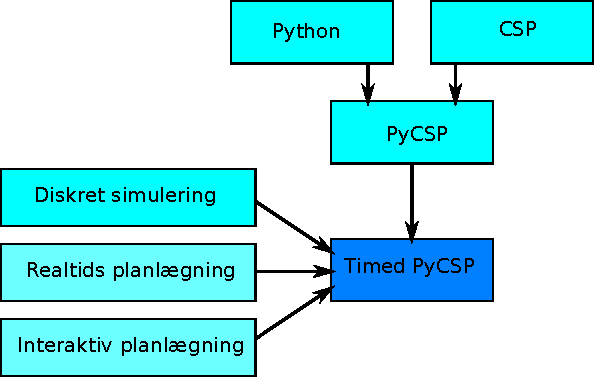
\includegraphics[scale=0.8]{images/intro}
	\caption{Samspil mellem CSP, Python og de tre anvendelsområder af tid samlet i Timed \pycsp .}
	\label{fig:intro}
\end{center}
\end{figure}

For hver model vil vi definere en række eksempler, der illustrerer disse anvendelsesområderne. Eksemplerne skal sikre den praktiske anvendelighed og senere bruges til at vise, hvordan et tidsspecifikt problem kan løses henholdsvis med og uden vores udvidelse. Eksemplernes formål er altså, at give et klart indblik i de krav, der stilles til en udvidelse af \pycsp, og hvilke fordele en introduktion af de givne anvendelsesområderne i \pycsp vil give. På denne baggrund vil vi komme med løsningsforslag som tager udgangspunkt i den praktiske anvendelighed. Disse løsningsforslag vil såfremt det er muligt, blive implementeret som en udvidelse af \pycsp.

Specialet vil derfor være struktureret som følger. I \autoref{chap:csp} vil vi gennemgå CSP og \pycsp med fokus på de dele der er relevante i forhold til at introducere tid. I \autorefs{chap:des}, \ref{chap:rtp} og \ref{chap:is} vil vi gennemgå de tre anvendelsesområder som beskrevet ovenfor. Afslutningsvis vil vi foretage en samlet i evaluering og konklusion i \autoref{chap:konklusion}.

%Mål: At lave en praktisk anvendelig udviddelse af pycsp, som kan bruges af udviklere til at løse problemer, der har en naturlig dimension af tid.

%Mål: At undersøge om det er muligt at lave en praktisk anvendelig udviddelse af pycsp, som kan bruges af udviklere til at løse problemer, der har en naturlig dimension af tid.

\section{Vores bidrag}
\fxwarning{Slet dette afsnit eller skriv noget}
\section{Termer}
I forbindelse med dette speciale vil vi bruge følgende termer:
\begin{list}{}{}
\item \textbf{\Sched} dækker over det engelske ord Scheduler. En \sched~ er det software der står for at planlægge i hvilken rækkefølge processerne skal udføres på computeren.
%\item \textbf{Tidsdomænet} Tidsdomænet er den overordnede .... \fxwarning{Hvad fanden skal der stå her}
\item \textbf{Realtid} er en tidsmodel, der i litteraturen også er defineret som absolut tid, eller Newtonisk tid. Tiden ses som en fundamental struktur i universet, der 
fremskrives kontinuerligt og uafhængigt af nogle eksterne kræfter.
\item \textbf{Diskret tid} er en anden tidsmodel. Her samples værdier fra den kontinuerlige tid, således at tiden fremskrives i ryk. Den enkelte sample er normal taget med et konstant tidsinterval, men kan også være taget med et variabelt tidsinterval. I diskret tid kan tiden enten drives frem af tiden selv, som i realtid, eller fremskrives manuelt. I dette speciale defineres diskret tid til at have variable tidsintervaller, og skal fremskrives manuelt.
\item \textbf{Anvendelsesområde} er en konkret implementation af en tidsmodel.
\item \textbf{\code{Skrivemaskine-font}} markerer i dette speciale variabelnavne, funktioner,  klasser og moduler som findes i koden. 
\end{list}




\chapter{CSP og PyCSP}
CSP er et sprog til at beskrive uafhængige processer, der udelukkende udveksler information ved at sende og modtage beskeder over eksplicitte kanaler mellem processerne. Det blev introduceret af \citeauthor{hoare-csp} i \citetitle{hoare-csp}\cite{hoare-csp} og ligger til grund for adskillige praktiske implementationer i et udvalg af programmeringssprog, heriblandt Occam, Java, C++ og Python. I Python hedder udviddelsen PyCSP\cite{pycsp}, og er udviklet i et samarbejde mellem mellem Tromsø og Københavns Universitet, med henblik på at kombinere fordelene fra Python og CSP. 

\section{Kommunikation mellem processer}
Kommunikation mellem to processer i CSP kan kun ske når begge processer er klar til at kommunikere. Hvis den ene proces er klar før den anden er den nødt til at vente på at begge er klar. Herefter kan de kommunikere og så fortsætte. Selve kommunikationen foregår over kanaler. De nævnte implementationer har forskellige typer kanaler, set med henblik hvordan de forbindes til andre processer. Generelt findes der fire 4 typer af kanaler: one-to-one, any-to-one, one-to-any og any-to-any. Forskellen ligger i hvem og hvor mange der kan læse og skrive til en kanal. Det er klart at any-to-any kanalen er den mest generelle og har funktionalitet som de andre. Dette er udnyttet i bl.a. PyCSP hvor det er den eneste kanaltype der er til rådighed. Fælles for dem er at det skal specificeres om en proces skal kunne skrive eller læse fra en kanal\fxnote[inline, nomargin]{fact check på dette}. Hvis to processer skal kunne både læse fra, og skrive til hinanden, skal de have to kanaler for at opnå det. 

en \code{alternation} er en struktur til at foretage valg omkring kommunikation. En \code{alternation} kan indeholde et vilkårligt antal kanalender, samt eventuelt en \code{guard}. Når en \code{alternation} udføres foretages der således et valg mellem de kanaler der er klar eller \code{guarden}. En guard kan enten være en \code{timeout}- eller \code{SKIP-guard}. En \code{timeout-guard} er klar efter en angivent tidspunkt og en \code{SKIP-guard} er altid klar. Dette giver mulighed for konstruktioner som f.eks. "kommuniker hvis der er processer der ønsker at kommunikere med os, ellers fortsæt". 




\subsubsection{noter}
Kanaler, karakteristika for dem\\
Alternations, guards og andre vigtige strukturer\\
Tid i PyCSP\\

3 versioner af PyCSP - greenlets osv.\\
 - indsigt og valg af greenlets her\\

parallel, sequence, spawn\\
buffered channels\\
retire\\






\chapter{\des}
  \section{Beskrivelse/teori}
    \fxnote[inline]{Beskrivelse af tidsmodellen, teorien omkring den og 
    hvor/hvad den benyttes til. Teori: henvisning til litteratur, bl.a.  
    matematik/beviser for modellen}
    
\subsection{Barrierer}\label{barrier}
For at modellere tid i PyCSP, skal der foretages en 
række valg. I \des findes der i modsætningen til 
Parallel \des \fixme{referencer} en global tid og alle processerne skal derfor have  en 
fælles tid der tæller op samtidigt. Den mest brugte metode i CSP sammenhæng er 
at implementere en barrier som en selvstændig process. Eksempelvis kan den implementers som i \autoref{barrier-imp}.
%\begin{minipage}[b]{1\linewidth}

\begin{lstlisting}[float, label=barrier-imp,caption=En barrier i PyCSP]
@process
def Barrier(nprocesses, signalIN, signalOUT):
	while True:
		for i in range (nprocesses):
			signalIN()
		for i in range (nprocesses):
			signalOUT(0)
\end{lstlisting}
%\end{minipage}

Barrier blev introduceret i MPI, og sikrer at alle tråde har nået dette punkt 
før de må fortsætte. I PyCSP er det trivielt at have  denne egenskab, da 
processer til begge kanalender er klar, og med to kanaler kan man sikre at 
ingen proces modtager et signal før alle processer har sendt et signal til 
barrieren.
\fxnote[inline]{fortsættes med ulemper med barriere og generelt hvorfor vi 
skal holdes os fra det. noget med at man skal kalde barrieren to  gange}

\section{Eksempel}
\fxnote[inline]{Beskrivelse af eksemplet og hvordan det er relateret til problemet/modellen. Beskrivelse af løsning uden vores tid}


\subsection{Hajer og fisk på Wator} Som eksempel på en \des har vi valgt at tage 
udgangspunkt i det scenarie som A. K. Dewdney
beskrev i artiklen \cite{wator}. Artiklen beskriver den
fiktive planet Wator, der har form som en torus og er fuldstændig
dækket af vand. Verdenen er inddelt i felter \cite[s. 20]{wator}, og disse felter kan være tomme, indeholde en
fisk eller en haj. Følgende karakteristika beskriver fisk og hajers
opførsel.

\begin{itemize}
\item[Fisk]
Lever af plankton, en ressource som er uendelig. Hvis der er en ledigt 
tilstødende felt, bevæger en fisk sig til dette felt. Hvis der er flere ledige 
felter vælges et tilfældigt. Såfremt en fisk overlever 3 tidsskridt forplanter 
den sig.
\item[Hajer]
Såfremt der er fisk i et eller flere tilstødende felter, vil hajen bevæge sig 
til et af disse felter og spise fisken. Hvis der er ikke er nogen fisk i et af 
disse felter flytter hajen sig til et tilfældigt valgt ledigt felt. Hvis en haj 
ikke spiser i 3 tidsskridt dør den. Overlever den i 10 tidsskridt forplanter 
den sig.
\end{itemize}

For hvert tidsskridt vil alle fisk og hajer udføre en handling ud fra
ovenstående opførsel.
Til at initiere systemet skal der defineres en størrelse af verdenen,
samt hvor mange fisk og hajer der er til stede fra start. Disse fisk og
hajer placeres tilfældigt i verdenen.
Såfremt de initielle parametre for antal fisk og hajer understøtter en 
bæredygtig bestand forventer vi at se bestanden af henholdsvis fisk og hajer 
oscillerer afhængigt af hinanden.

\fxnote[inline]{Hvorfor har vi valgt dette eksempel. Hvorfor er dette eksempel 
relevant til brug i parallel computing. Hvorfor forventer vi at det kan gøres 
smartere med introdsuktionen af tid.}

Vi har valgt dette eksempel, da det er enkelt og let forståeligt, men samtidig 
introducerer problemstilinger omkring synkronisering når det paralleliseres.  
Disse problemstillinger optræder fordi en opdatering af hvert felt er afhængigt 
af de omkringliggende felter, og vil derfor være afhængig af felter fra andre 
processer i grænsetilfælde. Ud over at være afhængig af information fra andre 
processer, kan en opdatering også påvirke data hos andre processer. Dette er 
tilfældet hvis en fisk eller haj skal bevæge sig fra et område styret af èn 
proces til et område styret af en anden proces.  \fxnote[inline]{Noget om real 
world applikation?}

\subsubsection*{Før introduktion af et tidsbegreb i CSP} 
For at simulere Wator verdenen i et CSP-system hvori tidsbegrebet ikke er 
introduceret, er vi nødt til at udføre en synkronisering af de enkelte 
processers arbejde. Denne synkronisering kan ske ved brug af barrierer, hvor 
alle processer udfører en handling og mødes i barrieren før de fortsætter.

\fxnote[inline]{MAV af model, hvorfor ikke en bedre csp approch med forsendelse 
af shadowrows og totalt seperapelt data}
Vi har valgt at basere vores model på \cite{crew}, hvor verdenen repræsenteres 
som en delt datastruktur og adgangen til denne styres med barrierer. I vores 
model er hver proces derved ansvarlig for en del af verdenen og tilgangen til 
den delte datastruktur sker ud fra CREW-princippet (Concurrent Read, Exclusive 
Write) som angivet i artiklen, og styres vha. af barrierer. 

Vi deler verdenen lodret, hvor hver proces styrer en verdensdel. Hver proces 
gennemgår sin verdensdel og udfører en mulig handling for hver fisk og haj, dog 
vil fisk og hajer i de sidste to kolonner i hver verdensdel ikke bliver 
opdateret på nuværende tidspunkt. Dette skyldes at henholdsvis processen selv 
og den umiddelbar til højre for den, har skriverettigheder til disse to 
kolonner.
Når denne opdatering er fuldført mødes processerne i en barriere, hvorefter 
hver proces opdaterer de to sidste kolonner. Herefter mødes processerne igen i 
barrieren, og når alle kolonner er opdateret, kan der foretages en 
visualisering af de udførte opdateringer. Til slut mødes alle i en barrierer igen før processerne kan begynde en ny iteration \fxnote[inline]{pseudo kode eksempel?}

En representation af opdelingen ses på \autoref{fig:wator}. Her er verdenen 
opdelt mellem to processer, og de to kolonner mellem hver del opdateres i et 
seperat tidsskridt. Når disse to tidsskridt er udført kan der foretages en 
visualisering, hovrefter næste iteration af opdateringer kan begyndes.  

Vi har valgt denne model frem for en mere ren CSP model, da denne model 
klarlægger brugen af barrierer bedre. I en mere ren CSP-model ville man 
foretage en direkte udveksling af data mellem 
processerne,\fxnote[inline]{mere\ldots} 

\fxnote{konklusion hvordan var det at implementerer og hvor stor parallelitet kan man opnå. }

\begin{figure}
  \begin{center}
  \includegraphics[scale=0.75]{images/wator}
  \caption{Opdeling af verdenen mellem to processer. Der er for hver verdensdel 
  to kolonner som opdateres i et seperat tidsskridt.}
  \label{fig:wator}
  \end{center}
\end{figure}

\subsection{Kunder i en bank} Et klassisk eksempel inden for \des er at simulere  
en række kunder der alle ankommer til en butik, hvor de skal serviceres. Dette 
simple problem kan bruges til at modellere mange forskellige 
problemstillinger, som hvordan flowet ændrer sig hvis man varier en parameter 
i systemet. Programmeringssproget SimPy har som et af deres eksempel, en 
simulering af kunder i en bank. SimPy bruger dette som en gennemgående 
eksempler hvor de løbende udvider deres model for at vise forskellige 
egenskaber ved deres model. For at nemt at kunne sammenligne SimPy  med vores 
model vil vi bruge dette eksempel.

I det simple tilfælde af eksemplet ankommer der en kunde til banken på på et 
tilfældigt tidspunkt. Hun opholder sig i banken i et tidsrum, hvorefter hun 
igen forlader banken.

I det simple eksempel kan der ikke uddrages meget information, da banken ikke 
består af en begrænset ressource som kunderne skal tilgå.  Eksemplet er derfor 
også udvidet med en service disk, hvor alle kunderne skal betjenes af en 
servicemedarbejder. Alle kunder ankommer til banken i tilfældig orden og 
stiller sig i kø til at blive serviceret. Dette  svare til en M/M/1\fixme{hvad  
er en m/m/1 kø} kø.
\textbf{Uden tid}\fxnote{bedre overskrift}
I SimPy er kunderne en proces og det vil derfor være nærliggende ligeledes at 
modellere eksemplet i PyCSP med kunder som en proces. i SimPy kalder 
generatorfunktionen kunderne og kan kører den parallelt med sig selv. 
I PyCSP\fxnote{hvorfor?- kan man lave child processes der køre i samme 
parallel kald som dets parent?}, er standard metoden\fxnote{set fra 
kodeeksempler} at modellere mere statiske objekter, med en source og sink 
process og lade arbejdet flyttes mellem processerne. Derfor er modellen ændret 
så  generatorprocesen stadigt fungere som en source, men vi introducerer en 
bankproces som sink, og lader kunderne være arbejdet der flyttes mellem dem. 

Mens SimPy  kalder kundeprocessen og lader denne stå for håndteringen af 
kunden og tiden hun befinder sig i banken, har bankprocessen i PyCSP ikke 
mulighed for at kende tid og skal derfor selv holde en liste med kunderne 
i banken og  til hver tidskridt vide hvilke af kunderne der skal forlade 
banken. 

Tiden er igen modelleret ved brug af barrier se afsnit \vref{barrier}, men 
i stedet for  at kalde barrierens to krævede kald, lige efter hinanden, som 
normalt, for at være sikker på vi er i samme tidsskridt lader vi bank
processen gå ind i barrieren i starten af tidsskridtet, og så modtage kunder, 
indtil banken modtager et kald om at forsætte til næste tidsskridt af 
barrieren.
\begin{lstlisting}[float,label=bank-alternation-imp,caption=Modtage en kunde eller 
	barrier i Bankprocessen]
while True:
		(g,msg) = Alternation([{
		barrierREADER:None,
    customerREADER:None
    }]).select()
		if g == barrierREADER:
			break
    elif g == customerREADER:
			heappush(customers,(time+msg.waittime,msg))
\end{lstlisting}
Dette er smart, og nødvendigt for at lade banken have mulighed for at modtage 
et vilkårligt antal kunder i samme tidsskridt, samt vide hvornår der ikke vil  
komme flere kunder. Vi kan ressonere os til at barrieren stadigt virker efter 
hensigten ved at indse at for at generatoren kan komme foran med et tidsskridt og sende en 
kunde i et forkert tidsskridt skal den have fuldført begge begge kald til barrieren, men 
barrieren vil ikke modtage et kald fra nogle før det har kaldt bankprocessen, 
og derfor må generatoren vente i sit første kald til barrieren indtil banken har 
modtaget sit kald fra barrieren. 

For at kunderne kan tilgå den samme begrænsede ressource kræves en kø, og denne kan i PyCSP modeleres på flere måder, afhængigt at hvilken proces der skal have ansvaret for at vedligeholde køen. En metode er internt i en proces at have en liste, og lade det være processen ansvar. Processen med ansvaret kan så enten være den begrænsede ressource, eller en separat proces hvis eneste formål er at vedligeholde køen. For nyligt er der i PyCSP blevet introduceret ''buffered channels'', og man kan også vælge at bruge disse som en kø. Dermed kan man modellere sin ressource og lade den læse fra kanalen når den er klar uden at skulle beskæftige sig med køen. I eksemplet 
  \section{Design og implementation}
    \fxnote[inline]{Beskrivelse af design med udgangspunkt i eksemplet}
    \subsection{Scheduler}
Med valget af greenletversionen som grundversionen, og med henblik på at hovedparten af vores ændringer vil være i scheduleren, vil vi kort gennemgå denne.

\begin{lstlisting}[firstnumber=132,stepnumber=5,numbers=left, float, label=fig:scheduling, caption=Uddrag af Scheduler.py i greenletsversionen.]
    def getInstance(cls, *args, **kargs):
        '''Static method to have a reference to **THE UNIQUE** instance'''
        if cls.__instance is None:
            # (Some exception may be thrown...)
            # Initialize **the unique** instance
            cls.__instance = object.__new__(cls)

            # Initialize members for scheduler
            cls.__instance.new = []
            cls.__instance.next = []
            cls.__instance.current = None
            cls.__instance.greenlet = greenlet.getcurrent()

            # Timer specific  value = (activation time, process)
            # On update we do a sort based on the activation time
            cls.__instance.timers = []

            # Io specific
            cls.__instance.cond = threading.Condition()
            cls.__instance.blocking = 0
\end{lstlisting}

 I \cref{fig:scheduling} ses et uddrag af initialiseringskoden. Dels findes der tre lister af processer som scheduleren har mulighed for at vælge imellem når der skiftes proces.  
 \begin{list}
 \tightlist 
 \item \code{new}: Initeres på linje 140, og består af processer som lige er blevet scheduleres for første gang.
 \item \code{next}: Initeres på linje 141, og indeholder de processer der er klar til at blive kørt, og som har været kørt før.  
 \item \code{timers}: Initeres på linje 147, og indeholder de processer der har tilknyttet en timeout. De skal først scheduleres på et senere tidspunkt og venter dermed blot. Hvert element i listen består både af processen samt et tidsstempel for hvornår processen skal genaktiveres. Denne liste bliver gensorteret hver gang der indsættes en ny proces.
 \item \code{blocking}: Initieres på linje 150, og er en variabel.Processer der venter på IO operationer, er ikke klar til at blive scheduleret, men heller ikke afsluttet. Scheduleren kan derfor ikke schedulere dem, men holdes styr på antallet af ventende processer vha. denne variabel, for at kunne afgører om Scheduleren skal afslutte eller afvente.
\end{list}

Når \sched en er startet, itererer den igennem alle tre lister, indtil de alle er tomme, og der ikke er nogle processer der er blokeret. Dette betyder at der ikke længere kan komme processer der ønskes at blive lagt på \sched en, og den kan dermed afslutte.

For at markere at vi ikke kun skal foretage en planlægning
af processerne, men foretage en simulering, har vi lavet en
\code{Simulation} klasse der arver fra \code{Scheduler}. Alle ændringer
vi skal foretage for at gå fra en almindelig \sched ~til en simulerings
\sched, vil således indkapsles i denne klasse, mens alt hvad de to
klasser har til fælles vil være isoleret i greenlets versionen af
\code{Scheduler} klassen. Dette har yderligere den fordel at man tydeligt kan se
at alle klasserne i simulation versionen arver en simulerings \sched ~og
ikke \code{Scheduler} fra greenletsversionen.

%\fxnote{dårlig overskrift}{\subsection{Repræsentation af tid}} Vi
%vil i dette afsnit gå i dybden med listen \code{timers} der findes i
%klassen \code{Scheduler}, samt se hvordan den kan inkorporeres i vores
%design.

\subsection{Tid i greenletsversionen} I \pycsp foregår kommunikation
kun når begge kanalender er klar dvs. når der både findes en
kanalende der vil skrive og en kanalende der vil læse. Hvis
kun en af kanalenderne er klar, vil den vente indtil der findes
minimum en kanalende af hver type, der er klar. Dette medfører
risikoen for at processen aldrig kommer videre, men går i deadlock.
I \pycsp har man derfor i \code{alternation} mulighed for at
tilknytte en timeout til en \code{guard}. Dette giver mulighed for
at en proces, kun er villig til at vente på kommunikation i en
given tidsperiode. 
\begin{lstlisting}[float=hbtp, label=Timeout,caption=Timeout i Alternation (fra dokumentationen til PyCSP)]
Alternation([{Timeout(seconds=0.5):None}, 
             {Cin:None}]).select()
\end{lstlisting}

I \cref{Timeout} ses et minimalt eksempel hvor processen kun er villig
til at læse fra kanalenden \code{Cin} i $0.5$ sekunder. Hvis ikke der
er modtaget en besked indenfor 0.5 sekundt, accepteres timeoutguarden
og processen er ikke længere villig til at læse fra \code{Cin}, og
fortsætter sin kørsel.

Tid er dermed blevet introduceret i \pycsp, men kun for at at have
mulighed for at tilknytte timeout til en \code{alternation}. Vi ønsker
at videreudvikle denne struktur til at håndtere tidsdelen for alle
processer, samt for at fungere med diskret tid, modsat den eksisterende
løsning hvor tiden er kontinuerligt.

\subsection{Timers}  
Vi forventer at brugen af
listen \code{timers}, vil øges betragteligt og at den gennemsnitlige
længde af listen vil stige, når der udvikles simuleringsproblemer. Dermed 
øges kravet om en effektiv implementation af \code{timers}\fxnote{skal 
vi evaluere om dette rent faktisk forbedrer ydelsen}. 

For at forbedre ydelsen af \code{timers} listen, 
ændrer vi den fra en almindelig liste, til en min"-hob. En hob har
flere fordele ved skemaplanlægning og er nævnt i introduktionen til Pythons implementation af en hob\fxnote{ref til http://docs.python.org/dev/3.0/library/heapq.html}. 

Da en implementation af en hob
allerede findes i Pythoni modulet \code{Heapq}, som er effektivt implementeret i C, vælger vi at bruge denne. Den eneste handling
der ikke er som standard er implementeret, er fjernelsen af et arbitrært element
fra hoben. Dette sker i den eksisterende løsning når en proces
aktivere et andet valg i \code{alternation} end timeout. I dette tilfælde skal
processen ikke vente på sin timeout, men elementet skal fjernes fra
\code{timers} listen. For at fjerne et element i en hob, må man som i
en normal liste lave en lineær søgning i hoben, og derefter genoprette
hob"-egenskaben i listen. Dette vil dog ikke tage længere tid end det
allerede tager da en fjernelse af en timeout i greenletversionen på nuværende
tidspunkt bruger en lineær søgning, til at finde elementet der skal
fjernes, og genoprettelsen af hobegenskaben også tager lineær tid \inline{ref til construction of heaps can be done in linear time using Tarjas algorithm.\\$http://en.wikipedia.org/wiki/Tarjan\%27s\_algorithm$}For at se en forskellen mellem greenletversion der bruger en liste og simulationsversionen der bruger en hob kan man sammenligne \cref{sched_timer} linje 205 med \cref{sim_timer} linje 126.


\subsection{Diskret tid} For at konverterer greenletversionen der knytter sig til reel tid, skal vi ændre de steder som bruger tid. Som vi har beskrevet tidligere er det eneste sted tid er introduceret i forbindelse med timeout og dermed i listen \code{timers}. Vi kan dermed nøjes med at ændre de steder i \sched en som indvolvere \code{timers}. Det første sted hvor timers indgår er i udvælgelsen af hvilken proces skal vælges(\cref{sched_timer}). Her sammenlignes på linje 204  første tidsværdi i timers, med det nuværende tidspunkt i time klassen. Hvis det nuværende tidspunkt er større end værdien i timers udvælges denne proces til at køre næste gang og fjernes fra timers listen.

Da tiden er diskret, og kræver et aktivt valg før den skifter kan vi tilføje en yderligere begændsning i forhold til greenletsversionen. For simuleringsversionen skal tiden være præcist det der er angivet i \code{timers}, før processen skal aktiveres, og ikke kun størrer end som angivet i greenletsversionen.  Simuleringsversionen af den del der foretager udvælgelser en proces fra  \code{timers} kan ses i \cref{sim_timer}. 

\begin{figure}[hbtp]
\begin{minipage}[c]{\linewidth}
\begin{lstlisting}[firstnumber=204, label=sched_timer, caption=Udvælgelse af proces fra listen timers (fra scheduling.py)]
if self.timers and self.timers[0][0] < time.time():
  _,self.current = self.timers.pop(0)
  self.current.greenlet.switch()
\end{lstlisting}
\end{minipage}
\begin{minipage}[c]{\linewidth}
\begin{lstlisting}[firstnumber=124, label=sim_timer, caption=Udvælgelse af proces fra listen timers (fra simulation.py)]
if self.timers and self.timers[0][0] <= Now():
  assert self.timers[0][0] == Now()
  _,self.current = heapq.heappop(self.timers)
  self.current.greenlet.switch()
\end{lstlisting}
\end{minipage}
\end{figure}



\subsection{Funktionerne Now og Wait}
 I Python kan man benytte modulet
\code{time}, hvis man ønsker at introducer begrebet tid. Med dette
modul kan man få af vide hvad klokken er. fra en brugers synsvinkel
repræsenteres tiden som kontinuerlig, og hver gang en bruger spørge
om klokken, fås et bestemt tidspunkt. Med computere findes tid som
kontinuerligt begreb ikke, men derimod er tiden internt repræsenteret
som diskrete tidsskridt. Størrelsen af disse tidsskridt varriere
af bla. hvilken computer programmet køres på og operativsystem.
Når vi ønsker at introducere \des skal det ikke ses som diskret
modsat kontinuerligt, men at de enkelte tidsskridt i \des er af
variable størrelse modsat i modulet \code {time} der har en konstant
størrelse. Da man i \code{time} modulet har en fast tidsskridt og
tid i det kontinuerlig tifælde også er inddelt i faste størrelse
som eks. sekunder, kan man med time modulet måle tidsintevaller der
korrespondere med den kontinuerlige tid. I \des findes der ikke en
sammenhæng mellem den kontinuerlige tid og dens egen repræsentation af
tid. For \des er tid derimod blot et tal der starter som 0, og stiger
i abitrærer tidskridt. Når tiden i \des på denne måde er afkoplet
en relation almindelig tid, kan man heller ikke snakke om at et tidsrum
har sekunder eller timer. I \pycsp kan man i timeout planlægge en
begivenhed til at ske om f.eks. 5. sekunder. I \des findes sekunder som
begreb ikke, men man kan angiver at når tiden er talt op med 5 skal
begivenheden ske. \inline{Skal dette splittes op og halvdelen skal i
teori?}

Når et problem modeleres i \des, vil der altid være behov for at
tilføje en sammenhæng mellem tid i problemet og et tid i modellen. Da
der der ikke findes en fast sammenhæng, skal modellen derfor eksplicit
definere om 5 sekunder skal repræsenteres som, at tiden internt i
\pycsp tælles op med 5, 0.5 eller 0.05.

Vi har valgt at repræsentere tiden som en intern variabel i \sched.
Dette kan vi gøre da \sched ~er en singelton og der findes derfor kun
en variabel med tid. For processer der ønsker at kende tiden har vi
introduceret funktionen \code{Now()} der returnere hvad tiden er på et
given tidspunkt.

\inline{På det teoretiske plan snakker vi om at planlægge
begivenheder, mens vi i implantationen snakker om Wait og at ''stalle''
en process }

I programmeringssproget \simpy lader man en proces vente ved at
foretage kaldet \code{yield}. Dette yield sørger for at processen ikke
fortsætter før et foruddefineret tidsrum er gået.

\begin{lstlisting}[firstnumber=11 , stepnumber=2, numbers=left,float=hbtp, label=yield, caption= Et yield i \simpy (Taget fra Bank05.py i eksemplet fra \simpy)] 
def visit(self,timeInBank): 
  print now(), self.name," Here I am" 
  yield hold,self,timeInBank print now(),
  self.name," I must leave" 
\end{lstlisting}

I \cref{yield} ses hvordan en kundeproces ankommer til banken,
printer tiden, foretager et yield, og når processen fortsætter
fra dette kald er tiden steget med værdien \code{timeInBank}.
Til slut printer processen igen tiden. Brugen af yield er knyttet
til implementeringen af \simpy og skyldes at \simpy implementere
hver process som en \code{corutine}. Vi skal i \pycsp have en
ligende mulighed for at lade en proces vente. Da dette allerede er
implementeret via timeout i greenlets versionen af \pycsp, kan vi
uden at ændre i den eksisterende \sched tilføje en ny funktion
\code{Wait} der fungere som timeout, men kan kaldes af processerne
på et vilkårligt tidspunkt. \inline{Dette skal måske ændres
da jeg ikke har talt med Rune om nødvendigheden af ''while now()<t)''. Og jeg har derfor ikke beskrevet i teksten hvordan funktionen virker.}

\begin{lstlisting}[firstnumber=20,float=hbtp, label=wait, caption=Wait i simuleringsversionen.] 
def Wait(seconds): 
  Simulation().timer_wait(Simulation().current, seconds) 
  t = Now()+seconds
  while Now()<t: 
    p = Simulation().getNext() 
\end{lstlisting}

Funktionen \code{Wait} er essentielt det eneste værktøj der skal til for at planlægge en begivenheder ud i fremtiden, og vi har på nuværenede tidspunkt en  simpel begivenhedssimulator der kører i reel tid. 

\subsection{Fra reel tid til diskret tid.}\label{sec:}
Vi ønsker sædvanligvis at en simulering, kan eksekveres uafhængigt af tiden der simuleres det vil sige at når der ikke sker flere begivenheder til et givent tidspunkt skal tiden fremskrives til det næste tidskridt hvor der sker en begivenhed og ikke kun med et fast tidsskridt. Modsat gælder det også at tiden ikke må tælles op før alle processer har indikeret at de ikke ønsker at foretage mere arbejde. 

I den eksisterende \sched ~ er tiden reel og indkrementeres derfor løbende uafhængigt af processernes tilstand. Dette kan illustreres med et eksempel; Proces 1 har startet en ny thread via et \code{io} kald, og er derfor blokeret. Proces 2 står i en \code{Alternation} med en timeout guard. Uafhængigt af tiden det tager proces 1 at komme ud fra sit blokerede kald, skal proces 2 vide at når timeout'en er indtrådt. Dette er implementeret i \cref{fig:blocking_sleep} på linjerne 242 til 251. For at nå disse linjer findes der processer der er blokeret samt processer der venter på en timeout. Nu startes en separat tråd der signalere \sched en, når næste begivenhed i \code{timers} listen indtræffer. \Sched en kan nu vente på et signal, som vil komme fra enten en blokeret proces eller den nyoprettede tråd.

Denne ekstra tråd til håndtering er tid i et blokeret kald er slet ikke nødvendigt i \des. For at tiden skal tælles op må ingen processer være blokeret; De skal i stedet enten have kaldt funktionen \code{wait} eller vente på kommunikation.  
Så længe der findes blokerede processer venter vi på dem, uden at tage hensyn til antallet processer i \code{timers}.

For at at simuleringen kan fortsætte skal tiden tælles op på et tidspunkt, og dette må gøres eksplicit at simulerings \sched en.  Kun i det tilfælde hvor der ikke findes nogle processer der kan planlægges vælger vi at tælle tiden op. Vi ved at der ikke kan foregå flere begivenheder til et tidsskridt når der kun findes processer i \code{timers} listen. Vi kan i det tilfælde finde tidspunktet for den næste begivenhed og sætte tiden til denne begivenhed. Følgende er implementeret i \cref{fig:sim_sleep}.
\begin{figure}[hbtp]
\begin{minipage}[c]{\linewidth}
\begin{lstlisting}[firstnumber=239, label=fig:blocking_sleep, caption=Uddrag af \sched en i \code{Scheduler}]
self.cond.acquire()
if not (self.next or self.new):
    # Waiting on blocking processes or all processes have finished!
    if self.timers:
        # Set timer to lowest activation time
        seconds = self.timers[0][0] - time.time()
        if seconds > 0:
            t = threading.Timer(seconds, self.timer_notify)
            # We don't worry about cancelling, since it makes no 
            #difference if timer_notify is called one more time.
            t.start()
            # Now go to sleep
            self.cond.wait()
    elif self.blocking > 0:
        # Now go to sleep
        self.cond.wait()
    else:
        # Execution finished!
        self.cond.release()
        return
self.cond.release()
\end{lstlisting}
\end{minipage}
\begin{minipage}[c]{\linewidth}
\begin{lstlisting}[firstnumber=158, label=fig:sim_sleep, caption= uddrag af \sched en i \code{Simulation}]
self.cond.acquire()
if not (self.next or self.new):
  # Waiting on blocking processes
  if self.blocking > 0:
    # Now go to sleep
    self.cond.wait()
  #If there exist only processes in timers we can increment
  elif  not (self.next or self.new or self.blocking): 
      if self.timers:
          # inc timer to lowest activation time
          self._t = self.timers[0][0]
      else:
          # Execution finished!
          self.cond.release()
          return
self.cond.release()  
\end{lstlisting}
\end{minipage}
\end{figure}

\subsection{Ting vi har stjålet fra \simpy.}
I vores implementering findes der i sagens natur i stort overlap med \simpy, som har været en inspirationskilde til hvordan et simuleringssprog kunne udvikles i Python. En del af arbejdet med \simpy har vi kunne bruge direkte i vore implementering, efter devisen om ikke at genskrive eksisterende god kode. Det drejer sig om funktionalitet til dataindsamling, bearbejdning og visualisering. I \simpy findes en \code{Monitor} klasse. Formålet med denne klasse er at gemme tid/værdi par. Dermed kan man efter endt simulering, analysere på hvordan værdierne ændret sig over tid.



  \section{Evaluering}
    \fxnote[inline]{Evaluering af hvordan eksemplet løses efter den valgte 
    implementation benyttes. Inkluderer test+performance}
  \section{Fremtidigt arbejde}
  \section{Opsummering}

\chapter{Real-time planlægning}
Vi vil i dette kapitel beskrive Real-time planlægning (RTP), samt diskutere hvordan det kan implementeres i \pycsp. 

RTP er baseret på den kendsgerning at nogle begivenheder i programmer kan være vigtigere at få udført end andre indenfor en afgrænset tidsperiode. Dette kan f.eks. være interrupts, input- eller output enheder eller interne processer. Med RTP tilknytter man en deadline for hver begivenhed, som bruges til at planlægge rækkefølgen for afvikling af begivenhederne. Formålet er at optimere antallet af begivenheder der når at blive udført inden deres deadline er overskredet. Normalt anses alle begivenheder for at være lige vigtige, og de planlægges ud fra en optimal udnyttelse af processoren. Denne optimale processorudnyttelse kan man være nødt til at gå på kompromis med hvis man ønsker at bruge RTP og derved prioritere visse begivenheder højere end andre. Man kan forestille sig en situation hvor man ikke starter en begivenhed med lav prioritet selv om den er klar, hvis man ved at en begivenhed med høj prioritet er klar kort tid efter, og venter derfor på at den er klar og igangsætter begivenheden med høj prioritet med det samme. 
RTP benyttes meget i specialiserede indlejrede systemer til f.eks medicinsk udstyr, kontrol af luftrummet, på rumstationen ISS\cite{Audsley1990} og mange andre steder. Det er dog også anvendeligt i mere gængse applikationer, typisk i forbindelse med en eller anden form for interaktion med den virkelige verden. 

I litteraturen omkring RTP bruges begreberne hard- og soft deadlines samt hard- og soft real-time systemer forskelligt, så vi vil i det følgende gennemgå hvordan vi definerer disse begreber. Vi har valgt at illustrere deadlines ved hjælp af time-value funktioner, hvor ``værdien'' indikerer det bidrag begivenheden bidrager med til systemets overordnede mål. 

\subsubsection{Kritisk deadline}
En kritisk deadline er en deadline som under alle omstændigheder skal overholdes for at opretholde systemets integritet. Såfremt en kritisk deadline overskrides vil der påføres skader på systemet som kan forårsage at systemets tilstand bliver udefineret. En kritisk deadline er illusteret på \cref{fig:hard-rtp}.

\begin{figure}
 \begin{center}
  
\includegraphics[scale=0.75]{images/critical-deadline}
	\caption{Begivenhed med kritisk deadline.}
	\label{fig:hard-rtp}
\end{center}
\end{figure}


\subsubsection{Hard deadline}
Vi definerer en begivenhed til at have en hard deadline såfremt en færdiggørelse af begivenheden efter deadlinen ikke tilfører systemet nogen positiv værdi. Modsat en kritisk deadline kan en overskridelse af en hard deadline accepteres. På \cref{fig:hard-dl} vises en hard deadline for en begivenhed. 

\begin{figure}
 \begin{center}
  
\includegraphics[scale=0.75]{images/hard-deadline}
	\caption{Begivenhed med hard deadline.}
	\label{fig:hard-dl}
\end{center}
\end{figure}
%Her tilføres der en positiv værdi til programmet hvis begivenheden afsluttes mellem dens starttidspunkt og dens deadline. Hvis begivenheden først er færdig efter deadline har den ingen værdi. En soft deadline (\cref{figure:soft-dl}) tilføjer den samme værdi som en hard deadline hvis begivenheden bliver færdig rettidigt. 

\subsubsection{Soft deadline}
Færdiggørelse af en begivenhed med en soft deadline til tiden tilføjer samme værdi til systemet som hvis den havde haft en hard deadline. Forskellen ligger i den tilførte værdi såfrem deadlinen overskrides. Hvor en hard deadline ikke tilføjer nogen værdi ved en overskridelse, vil en overskridelse af en soft deadline stadig tilføre en reduceret værdi ved færdiggørelse. Den tilførte værdi vil være omvendt proportional med længden af overskridelsen. \CRef{figure:soft-dl} illustrerer en soft deadline. 

\begin{figure}
 \begin{center}
  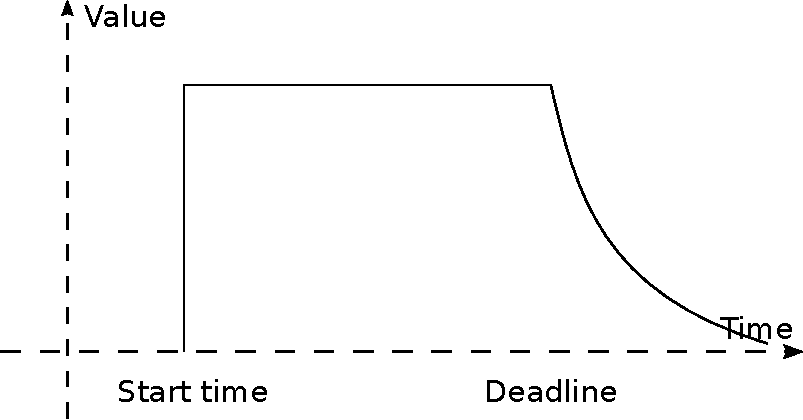
\includegraphics[scale=0.75]{images/soft-deadline}
	\caption{Begivenheden med soft deadline.}
	\label{figure:soft-dl}
\end{center}
\end{figure}


%Hvis deadlinen overskrides mindskes værdien den begivenhed tilføjer, omvendt propotionalt med overskridelsen. Ved en hard deadline er der ikke tilknyttet en egentligt %straf hvis en begivenhed ikke overholder sin deadline. Dette er derimod tilfældet i \cref{fig:hard-rtp}, der viser en begivenhed der tilføjer negativ værdi ved overtrædelse af en deadline. Hvis den tilknyttede straf for ikke at overholde en deadline er større end en hvad programmet maksimalt kan opnå ved at overholde alle deadlines kaldes det et ``hard real-time system''\cite{Laprie1989}.

\subsubsection{Hard real-time system}
Et hard real-time system er defineret ved et system der har begivenheder med hard deadlines, og kan garantere at disse ikke overskrides. Ydermere skal systemet være derterministisk, så denne garanti kan gives på forhånd. Det giver ikke mening at snakke om kritiske deadlines i hard realtime systemer da de kun adskiller sig fra hard deadlines med henblik på konsekvensen af en overskreden deadline, hvilket per definition ikke må ske i et hard real-time system.  

\subsubsection{Soft real-time system}
Et soft real-time system kan indeholde alle typer deadlines men opstiller ikke nogen garantier for at de overholdes. Det vil typisk bruge en algoritme til at op- og nedprioritere hvilke deadlines der skal overholdes såfremt alle deadlines ikke kan overholdes.

Generelt vil der i et real-time system ikke være alle begivenheder der har den samme type af deadline. Nogle begivenheder har ingen deadline, nogle har en soft deadline, og få har en hard eller eventuelt en kritisk deadline. 
%For RTP skal kørslen planlægges så begivenhederne har den maksimale udnyttelse af tilgængelige ressourcer samtidigt med at så mange deadlines som muligt overholdes, hvor de vigtigte deadlines prioriteres højest. 
 
\section{Planlægning af begivenheder}
Planlægningen af hvilke begivenheder der skal køres hvornår, tager udgangspunkt i det overordnede formål med systemet. Generelt vil formålet være at minimere antallet af overskredne deadlines, men dette er sjældent det eneste kriterie der planlægges efter, ofte vil prioriteten for, og tiden det tager at udføre en begivenhed indgå i planlægningen. Eksempelvis vil man ofte prioritere at nå en kritisk deadline selv om det betyder at man overskrider to soft deadlines. 

%De fleste eksisterende real-time systemer arbejder på isolerede systemer, hvor planlæggeren har fuld kontrol over hele computeren. Derfor er hovedparten af forskningen indefor området gået til udarbejdelsen af specialiserede kerner og komplette operativsystemer\cite{damm1989real, jones1979staros, levi1989maruti,ramamritham14scheduling}. Vi ønsker i modsætning hertil ikke at udvikle en specialiseret kerne, men lade \sched en i \pycsp kunne planlægge processer efter bedste evne baseret på informationer den har om processerne.

For at foretage en planlægning af begivenheder der opfylder systemets formål bedst muligt, skal vi have så meget information om begivenheder som muligt - jo mere vi ved om dem jo bedre en planlægning kan der foretages. De relevante informationer i forhold til planlægningen er, hvornår en begivenhed forekommer, hvor lang tid den tager at udføre samt hvilken prioritet den har. 

Ud fra den tilgængelige viden kan der foretages en statisk eller dynamisk planlægning\cite{cheng1987scheduling}. Statisk RTP kræver at vi har alle de nævnte informationer om alle begivenheder. Herved kan vi på forhånd foretage en fuldstændig planlægning og allerede inden start have klarlagt om nogen deadlines vil blive overskredet. Såfremt vi ikke har alle informationer til rådighed, er vi nødsaget til at foretage en dynamisk planlægning. Dette vil ofte skyldes at vi enten ikke ved hvornår en begivenhed forekommer, eller at vi ikke har information om hvor lang tid der tager at udføre en begivenhed. I praksis vil det være svært at opstille eksakte værdier for hvor længe en begivenhed er om at blive udført og der benyttes derfor ofte estimater i stedet for. \fxnote{hvilken betydning har det at der benyttes estimater i stedet for eksakte værdier?}

%Overordnet kan begivenheder planlægges enten statisk eller dynamisk\cite{cheng1987scheduling}. I statisk RTP er alle begivenheder kendt på forhånd. Planlæggeren kan i dette tilfælde allerede inden start udregne om det er muligt at overholde alle deadlines. Alternativt planlægges begivenhederne dynamisk hvis der uregelmæssigt kan ankomme nye begivenheder der skal planlægges. 

%\fxnote{Motivationen her skal være at vi skal kende begivenheders frekvens og længde - skriv noget om det!}
%I realtidssystemer er næsten alle begivenheder cykliske, med enten en regelmæssig eller tilfældig frekvens. Begivenheder der forekommer med en regelmæssig frekevens kan være f.eks. være målinger der skal foretages med bestemte intervaller, hvor uregelmæssig frekvens ofte vil være tilfældet ved begivenheder der skal indtræffe som reaktion på udefrakommende input, f.eks. fejl eller alarmer. 

%\begin{shaded}
%Til planlægningen har planlæggeren behov for at vide hvor lang tid det vil tage at udføre en given begivenhed per periode, men da dette tal enten ikke er kendt eller fast for hver periode, bruges der ofte estimater. Dette medfører at en aperiodisk begivenhed kan ankomme på et vilkårligt tidspunkt og da planlæggeren kun har et estimat for tidsforbruget kan man  ikke tilknytte en ``hard deadline'' til aperiodiske begivenheder, da der altid findes en kæde af aperiodiske begivenheder der medfører en overskridelse af en deadline. 
%\end{shaded}

%\fxnote*{Dette skal måske flyttes eller omformuleres så vi ikke med det samme begrænses til dynamiske \sched}{I \pycsp kan der til alle tidspunkter tilføjes nye processer, og derfor vil vi kun beskæftige os med en dynamisk \sched. Desuden har man ikke med \pycsp fuld kontrol over hele operativsystemet. Mængden af processerkraft vi har til rådighed til kørsel af processerne vil derfor varriere uafhængigt af \pycsp, hvorfor vi heller ikke kan lave et pålidelig ``hard real-time system'', men fokusere på et ``soft real-time system''.}

\subsection{Metoder til skemaplanlægning}
Der findes adskillige metoder til at planlægge rækkefølgen af begivenheder. De adskiller sig fra hinanden med henblik på hvilke informationer der er til rådighed og hvad de optimerer efter. Vi har valgt at kigge på ``Rate monotonic algorithm''\cite{lehoczky1989rate,liu1973scheduling} og ``Earliest deadline first''\cite{liu1973scheduling} indenfor henholdsvis statisk og dynamisk skemaplanlægning.

Hvor processer isoleret set har behov for at udføre deres opgave inden deres deadline, har \sched en behov for kvantitativt at kunne organisere dem indbyrdes, således den til enhver tid kan vælge hvilken proces der skal udføres som den næste. Hovedformålet for en  \sched ~ er derfor at gå fra en række processer med tilknyttet deadline og eventuelt andre egenskaber til en prioriteret liste. \\
Der fokuseres i litteraturen på om en algoritme er stabil eller ej. Såfremt en algoritme er stabil vil man kunne definere en delmægnde af begivenheder, for hvilke man kan garanterer at de ikke overskrider deres deadline. 

\subsubsection{Rate monotonic algorithm (RM)}
RM er en statisk \sched, der fra start af udregner en prioriteret liste på baggrund af frekvensen af processens periode, dermed vil processer der oftet skal have udført deres periode en højere prioritet, end processer med lav frekvens. RM er todelt og i første del udføres før selve simuleringen udregnes  prioriteten for processerne, og udvælger hvilke processer der kan medtages i selve udførslen. Anden del står for udvælgelsen af processer  under simuleringen, og her vælges simpelt den proces med den højeste prioritet. 

Et problem for RM er at ved udvælgelsen af processer der kan medtages har man ikke en optimal udnyttelsen af processorkraft. \Citeauthor{lehoczky1989rate} er kommet frem til at ``worst-case'' er udnyttelsen i gennemsnit 88\\cite{lehoczky1989rate}. Et større problem i relation til implementering i \pycsp er dog at RM er dog at den er statisk. Til gengæld er algoritmen stabil ved en overskridelse af deadline for en proces. 

\subsubsection{Earliest deadline first (EDF)}
Som alternativ til den statiske \sched, hvor man ikke kan ændre prioriten af processen løbende gennem simuleringe, findes de dynamiske \sched er, hvor er EDF er et eksempel. Her evalueres prioriterne af processerne dynamisk igennem simuleringen og evaluere dermed løbende hvilke processer der skal udvælges. I EDF har den proces hvis deadline ligger tættest på højest prioritet og den hvis proces har længst til deadline den laveste prioritet. Aperiodiske processer kan i EDF indgå på lige fod med de periodiske da man til hvert processkift evaluere hvilken der har den nærmeste deadline, som både kan være en periodisk proces som en aperiodisk.

Udnyttelsen af processorkraft kan i EDF komme op på 100\, da alle processer bliver planlagt løbende i modsætning til RM der foretager et valg om en given proces kan planlægges.  Ulempen ved EDF er den ikke er stabil i det vi ikke har kontrol over hvilke processers deadline der bliver overskredet. Dette er specielt et problem hvis man har en en uhomogen samling processer hvor en mindre del er kritiske.

\subsubsection{Least Laxity(LL)}
LL er en modifikation af EDF. LL kigger på hvor lang tid en begivenhed tager at udføre sammenholdt med hvor lang tid der er til deadline for begivenheden. Laxity er defineret som deadline minus tiden det tager at udføre begivenheden. Laxity bliver altså et udtryk for hvor presserende det er at igangsætte en begivenhed for at den kan nå sin deadline. I LL bruges dette til at prioritere de begivenheder der har mindst laxity højest når begivenhederne planlægges. \\
\\
I systemer hvor begivenheder ikke er isolerede men kan have interne afhængigheder, kan der opstå det problem der hedder prioritetsinvertering\cite{sha1990priority}. Dette problem opstår hvis en begivenhed med høj prioritet er afhængig af en begivenhed med en lavere prioritet. Derved bliver begivenheden i praksis kørt med den lavere prioritet da den ikke er klar før begivenheden med lav prioritet er færdig. Problemstillingen kan vises klart med følgende eksempel. Forestil dig tre begivenheder ($B_0,B_1,B_2$)med prioriteterne $Pr_0>Pr_1>Pr_2$. Først udvælges $B_0$ da denne har højst prioritet, men stopper da den er afhængig af kommunikation fra $B_2$. Den næste begivenhed der udvælges vil være $B_1$, og dermed bliver $B_0$ unødigt forsinket mens $B_1$ kører.\\
En ofte benyttet metode til at undgå priotetsinvertering er priotetsnedarvning. Ved at benytte denne løsning vil en begivenhed med lav prioritet, som en begivenhed med høj prioritet er afhængig af, nedarve prioriteten fra den begivenhed der venter på den. Herved sikres det at begivenheder med høj prioritet ikke kommer til at vente unødigt på prioriteter med lav prioritet. \fxnote{flere løsninger på prioritetsinvertering bør nok nævnes.}


\chapter{Eksempler}

\section{Hajer og fisk på Wator} Som eksempel på en DES simulation
har vi valgt at tage udgangspunkt i det scenarie som A. K. Dewdney
beskrev i artiklen \fixme[inline]{reference}. Artiklen beskriver den
fiktive planet Wator, der har form som en torus og er fuldstændig
dækket af vand. Verdenen er inddelt i felter som beskrevet på side
20 i \fixme[inline]{ref}. Disse felter kan være tomme, indeholde en
fisk eller en haj. Følgende karakteristika beskriver fisk og hajers
opførsel.


Fisk - bevæger sig og forplanter sig Lever af plankton, en ressource
som er uendelig. Hvis der er et ledigt tilstødende felt bevæger en
fisk sig til dette felt. Hvis der er flere ledige felter vælges et
tilfældigt. Hvis en fisk overlever 3 livscykler forplanter den sig.


Hajer - jager og forplanter sig Såfremt der er fisk i et eller flere
tilstødende felter flytter hajen sig herhen og spiser fisken. Hvis der
er flere tilstødende felter med fisk vælges et tilfældigt. Er der
ikke nogen fisk i nærheden bevæger en haj sig på samme måde som en
fisk. Hvis en haj ikke spiser i mere end 3 livscykler dør den. Hvis en
haj overlever 10 livscykler forplanter den sig.

For hvert tidsskridt vil alle fisk og hajer udføre en handling ud fra
ovenstående opførsel.

Til at initiere systemet skal der defineres en størrelse af verdenen,
samt hvor mange fisk og hajer der er til stede fra start. Disse fisk og
hajer placeres tilfældigt i verdenen.

Såfremt de initielle parametre understøtter en bæredygtig bestand
forventer vi at se bestanden af henholdsvis fisk og hajer oscillere
afhængigt af hinanden.

\section{Kunder i en bank} Et klassisk eksempel inden for \des

\section{Realtime planlægning i \pycsp}
\label{sec:rtp-pycsp}
\fxnote{(Flyttet fra RTP overordnet) Husk at snakke om begrænsning af greenlets mht. parallelitet når vi arbejder i realtid}
Da vi ønsker at introducere RTP i \pycsp, er der er række forhold, som vi skal tage højde for. Vi vil i dette afsnit tage udgangspunkt i de ovenstående opstillede muligheder og sammenholde dem med \pycsp. 

I \pycsp kan vi anskue processerne som begivenheder og derved bruge skemaplanlæggeren i \code{greenlets}-versionen til at styre hvilken proces og dermed hvilken begivenhed, der udføres. Vi har ikke umiddelbart informationer om, hvor lang tid en proces er om at blive udført, og det vil kræve en analyse af den enkelte proces at udlede estimater for det. Vi har valgt at fokusere på selve planlægningen af processerne og ikke på analysen. Dermed har vi ikke mulighed for at benytte RM og LL algoritmerne, da de begge benytter information om udførselstiden for en proces. Derved har vi EDF tilbage som mulighed, hvilket vi i det følgende vil implementere. En udvidelse af \pycsp til at benytte EDF er forholdsvis ligetil. Der skal laves en mulighed for, at brugeren kan angive en deadline til en proces, og vi skal ved kontekstskift sikre, at vi aktiverer den proces, der har den førstkomne deadline. Såfremt en deadline overskrides, skal vi have funktionalitet, til at håndtere dette. 

\pycsp har per definition interne afhængigheder mellem processerne i form af kommunikation over kanaler, og vi kan derfor opleve problemer med prioritetsinvertering. Den eneste metode til håndtering af dette, der kan bruges sammen med \pycsp, er prioritetsnedarvning, da de andre metoder forudsætter prioritetsinverteringen  sker som resultat af tilgang til kritiske regioner og ikke pga. kommunikation. Vi skal derfor også implementere prioritetsnedarvning for at sikre os mod prioritetsinvertering. 

Da vi benytter os af \code{greenlets}-versionen af \pycsp arbejder vi med en skemaplanlægger, der ikke kan foretage preemptive kontekstskift. Dette kan lede til problemstillinger som det er illustreret på \cref{fig:edf-nonpreemptive}. En metode til at mindske denne type problemer er at lade de enkelte processer afgive kontrollen med jævne mellemrum. Herved vil der blive foretaget en ny evaluering om hvilken proces, der skal aktiveres, og hvis der er processer, der har en nærmere deadline, som er blevet klar, aktiveres en af disse. Dette beror helt og holdent på at hver enkelt proces frivilligt afgiver kontrollen og gør det med jævne mellemrum, når den er aktiv. Dette betyder, at det er overladt til udvikleren at indsætte det på relevante steder i processens kode. 

\subsection{Tilknytning og overskridelse af deadlines}
Som udgangspunkt skal vi kunne håndtere, at en proces kan have forskellige typer deadlines. Umiddelbart er det oplagt, at der for hver proces tilknyttes en deadline samt hvilken type, det er. Dette giver mulighed for, at vi kan differentiere i den måde vi håndterer en overskreden deadline. F.eks. kan vi stoppe systemet helt i tilfælde af overskridelse af en kritisk deadline, kaste en exception ved en hard deadline og blot registrere overskridelser af soft deadlines. Uanset hvilken handling vi vælger at tilknytte til de respektive overskridelser, vil der altid være situationer, hvor den valgte handling ikke er optimal. 

Vi har derfor valgt en anden løsning, hvor en proces blot kaster en exception, hvis den overskrider en deadline. Dette overflødiggør, at der tilknyttes en specifik type deadline til en proces, da håndteringen af den kastede exception overgives til udvikleren. Det er herved op til den enkelte udvikler at definere, hvad der skal ske i hver enkelt proces, såfremt den overskrider en deadline. Dette giver den største frihed til at tilpasse håndteringen til den enkelte proces og applikation. 

\subsection{Udvælgelse af proces}
Udvælgelsen af hvilken proces der skal aktiveres, ved et kontekstskift, er givet ud fra vores valg af EDF. Som beskrevet i \cref{sec:edf} specificerer EDF, at det altid processen med den nærmeste deadline der skal aktiveres. For at opnå dette kan vi benytte stort set samme metode som vi brugte i \des. I \des sorterede vi processerne efter hvilket tidskridt de skulle aktiveres i, her kan vi sortere dem ud fra deres deadline.  

\subsection{Kanalkommunikation}\label{sec:rtp-kommunikation}
I litteraturen for  RTP fokuseres der kun på udvælgelsen og planlægningen af processer i \sched en. I \pycsp er kommunikation blokerende, hvilket betyder at fra en proces, ønsker at kommunikere, er den blokeret, indtil kommunikationen er gennemført. Ved one-to-one kanaler, er der kun en proces i hver ende, og derfor er  processen garanteret at gennemføre kommunikationen når modparten er klar til at kommunikere. Har processerne forskellige prioriteter risikere man prioritetsinvertering, og kan afhjælpe det med prioritetsnedarvning. 

I \pycsp er one-to-one kanalerne blevet fjernet, og erstattet af any-to-any kanaler, der ud fra et teknisk synspunkt er mere generelle og kan alt som one-to-one kanalerne kan. I any-to-any kanalerne er man ikke begrænset til kun at have en proces i hver ende af kanalen, men der kan være et vilkårligt antal processer. 
Benyttes prioritetsnedarvning på any-to-any kanaler, er man ikke som ved one-to-one kanaler sikret at det  processen der startede  prioritetsnedarvningen der får gavn af den, da parringen mellem processer der ønsker at kommunikere i \pycsp tilfældigt. Når processer kommunikere i  any-to-any kanaler kan man derfor med fordel sikre at det altid foregår mellem de to processer der har den højeste prioritet.


\subsection{Prioritetsnedarvning}\label{sec:rtp-pycsp-nedarvning}
At introducere prioritetsnedarvning i \pycsp virker umiddelbart ligetil, idet vi kan se de indbyrdes afhængigheder klart ud fra forbindelserne gennem kanalerne. Der kan forekomme andre afhængigheder, som er mindre synlige, men vi mener ikke disse vil forekomme i velskrevne CSP applikationer, og vi har derfor valgt at begrænse os til afhængigheder repræsenteret vha. kanaler. På trods af den umiddelbare simplicitet skal vi overveje hvornår, hvem og hvor længe, der skal arves i forbindelse med prioritetsnedarvning.

\subsubsection{Ændring af prioritet}
\label{sec:aendring-af-prioritet}
Vi arbejder med et dynamisk system af processer, hvor en proces, på baggrund af sin tilstand, er afhængig af forskellige andre processer for at kunne arbejde videre. 
Hvis vi højner prioriteten på alle processer, der er forbundet til en proces med høj prioritet, vil mange af processerne, der arver den høje prioritet, reelt ikke kunne bidrage til udførelsen af den proces, der starter med høj prioritet. Det er en bedre løsning, at det kun er den eller de processer, der kan sikre videre udførsel af den aktuelle proces, der tildeles højere prioritet. Hvis eksempelvis en proces med høj prioritet ønsker at skrive på en kanal, skal alle processer, der læser på den kanal, arve den høje prioritet, men de processer, som ønsker at skrive til en anden kanal, som processen med høj prioritet læser fra, skal ikke arve den høje prioritet. Generelt set betyder det, at der kun skal udføres prioritetsnedarvning, såfremt en højt prioriteret proces venter på at kommunikere, uden der er andre processer, der er klar til at indgå i den ønskede kommunikation. 

Vi har nu begrænset os til, at det kun er de processer der kan indgå i kommunikation over en kanal, der arver en prioritet. Med any-to-any kanaler findes der dog et vilkårligt antal processer i hver kanalende, og man risikerer en prioritetsdevaluering ved at lade flere processer arve en høj prioritet. I klassisk \csp findes der modsat hertil one-to-one kanaler, hvor man er sikret at det kun én proces' prioritet der bliver højnet ved prioritetsnedarvning. Forskellen kan illustreres af \autoref{fig:one-to-one-inheritance} og \cref{fig:any-to-any-inheritance}\fxwarning{tjek sidenr. er korrekt for de to figurer inden aflevering}. På \autoref{fig:one-to-one-inheritance}, bliver en proces' prioritet hævet fra fem til 10. Modtageren kan uden afbrydelser arbejde hen mod at kunne kommunikere, da afsenderen venter. I \autoref{fig:any-to-any-inheritance} bliver alle tre processers prioritet hævet til 10 og de vil skulle kæmpe mod hinanden for komme frem til en tilstand hvor de ønsker at kommunikere. 

\begin{figure}
 \begin{center}
  
\includegraphics[scale=1.00]{images/one-to-one-inheritance}
\caption{Procesnetværk med en afsender og en modtager. Afsenderen har prioritet 10, mens modtageren har en initiel prioritet på fem. Modtageren  får via prioritetsnedarvning hævet sin prioritet til 10. (Højere er bedre)}
  \label{fig:one-to-one-inheritance}
  \end{center}
\end{figure}

\begin{figure}
 \begin{center}
  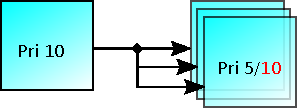
\includegraphics[scale=1.00]{images/any-to-any-inheritance}
  \caption{I dette eksempel findes der tre modtagere, som alle får hævet deres prioritet til 10.}
  \label{fig:any-to-any-inheritance}
  \end{center}
\end{figure}

Prioritetsnedarvning i et miljø med any-to-any kanaler har dermed en risiko for at medføre prioritetsdevaluering. Man kan forstille sig forskellige metoder til at eliminere eller minimere problemet f.eks ved at begrænse antallet af processer, der kan modtage en prioritetsnedarvning. Dette kunne gøres ved kun at lade en enkelt proces arve prioriteten,  men så skal man tage stilling til, hvilken proces, der skal udvælges. Dette kunne være den proces, der er tættest på at indgå i kommunikationen.  Udvælgelsen af processer må dog bero på en analyse af den enkelte applikation og dens aktuelle tilstand. Da vi ikke ønsker at begynde på en analyse af brugerens kode, må vi nødvendigvis sende prioritetsnedarvningen til alle processerne på kanalen. For at løse problemet vil vi i stedet fokusere på at minimere antallet af processer, der starter prioritetsnedarvningen, og det tidsrum processerne har arvet en prioritet.

Når kommunikationen på kanalen er gennemført, befinder processens sig i en anden tilstand og er afhængig af noget andet for at komme videre i sin udførsel. 
Når det midlertidige afhængighedsforhold ophører skal processer der har arvet en prioritet miste denne. Der skal selvfølgelig tages højde for at en proces kan arve forskellige prioriteter fra forskellige andre processer, så det skal være muligt at falde tilbage til den næsthøjeste arvede prioritet, i stedet for blot at skifte tilbage til den oprindelige prioritet. 

\subsection{Alternation}
Det er dog ikke kun i forbindelse med almindelig kommunikation vi skal forholde os til introduktionen af processer med et prioritet. I kodestrukturen \code{alternation}
 har en udvikler mulighed for at foretage et  prioriteret valg mellem flere forskellige kanaler. Et prioriteret valg mellem flere kanaler, kan dog være i konflikt med de processer som får opfyldt deres kommunikation. 
  
\citeauthor{Burns1990} beskriver og illustrerer præcist denne problemstilling i \citetitle{Burns1990}\cite{Burns1990}. Til at illustrere problemet beskriver de et eksempel, som er vist i \cref{lst:pri-select}. Denne kodestump viser et prioriteret valg mellem kanalerne A1 og A2. Til hver kanal er tilknyttet en proces, P1 og P2. Disse to processer har en prioritet tilknyttet på hhv.  Pri1 og Pri2. \CRef{tab:prioritizedSelect} viser hvilken kanal der bliver valgt, afhængig af processernes prioritet.

\begin{lstlisting}[firstnumber=1 ,float=hbtp, label=lst:pri-select, caption={(priority) select. Eksemplet er kopieret fra \cite{Burns1990}}]
(priority) select
   A1 -- Process P1
 or
   A2 -- Process P2
 end select
\end{lstlisting}

\begin{table}[htbp]
	\centering
	\begin{tabular}{lccc}
       	\toprule
                        & Pri1 > Pri2 & Pri1 = Pri2 & Pri1 < Pri2\\
        \midrule
	    priority select & A1          & A1          & ?  \\
        \bottomrule
        \end{tabular}
    \caption[]{Konflikten ved brug af prioriteret valg og procesprioriteter. Eksemplet er kopieret fra \cite[160]{Burns1990}}\\
    \label{tab:prioritizedSelect}
\end{table}

Man kan af \cref{tab:prioritizedSelect}  konstatere at der opstår en konflikt i kolonne tre, hvis udvikleren foretrækker en kanal, hvor den  tilknyttede proces' prioritet er lavere  end den anden proces'  prioritet. Man vil ikke kunne opfylde begge krav om både at kommunikere med den proces med højst prioritet, og lade udvikleren bestemme kanalen. For \citeauthor{Burns1990} er løsningen en ``orthogonal solutions'', der håndterer begge typer prioriteter. De ønsker overordnet set to typer udvælgelsesmetoder, weak- og strong Select. Weak select sorterer primært efter processernes prioritet og sekundært efter det prioriterede valg. Strong select udvælger udelukkende processer efter det prioriterede valg. De forstiller sig, at weak select skal bruges som den primære metode, men i specielle tilfælde skal en udvikler have mulighed for at tvinge et prioriteret valg igennem.

I artiklen fra \citeauthor{Burns1990} har de kun beskæftiget sig med one-to-one kanaler, og det er denne antagelse der medfører at et valg af kanal medfører et valg af en proces og dennes prioritet. Dette er ikke en mulighed i \pycsp hvor kanalerne er af typen any-to-any. Et valg af en kanal, medfører derfor ikke en direkte kobling til en proces, men til vilkårligt mange processer, der kan have individuelle  prioriteter. I \cref{sec:rtp-kommunikation} kommer vi frem til at kommunikationen altid skal sørge for at det er den højst prioriterede proces der kommunikerer. Dette kan bruges i \code{alternation} til at finde den højeste prioritet blandt de processer der er klar til at kommunikere, og bruge denne prioritet til udvælgelsen af kanal i \code{alternation}.

På baggrund af artiklen har vi valgt at \code{alternations} udfører en weak select, da denne version egner sig bedst til RTP . Vi vil i vores version ikke inkludere en strong select. Dette gør vi ud fra en betragtning om at den kun bør bruges i sjældne tilfælde,  da den vil modarbejde ideen bag RTP. Hvis en udvikler alligevel ønsker denne funktionalitet, vil har godt kunne opnå det i \pycsp, men vi ønsker ikke at tilskynde brugen, ved direkte at inkludere den.

\phantomsection
\label{misc:kanal-prioritet}
\subsubsection*{Prioritetsnedarvning i \code{alternations}}
Vi har som nævnt en klar kæde af afhængigheder i \pycsp men vi skal være opmærksomme på ikke at højne processers prioritet unødigt. Dette kan let blive tilfældet såfremt vi ikke holder ordentligt styr på, hvorfor en proces har den prioritet, den har, om den er sat af udvikleren, eller den er nedarvet. Man kan forestille sig en situation, hvor et uddrag af et proces-neværk består af en generator-forbruger-model med to generatorer og en enkelt forbruger. De to generatorer er forbundet til forbrugeren vha. en \code{alternation}, og har henholdsvis høj og lav prioritet. Eksemplet er illustreret på \cref{fig:alt-inheritance}. Forbrugeren vil i dette scenarium arve den høje prioritet fra den tilsvarende generator, men utilsigtet vil den høje prioritet derefter også propagere fra forbrugeren til generatoren med lav prioritet. Dette er ikke hensigtsmæssigt, da de to generatorer nu har lige høj prioritet og ikke det forhold, som udvikleren oprindeligt har angivet. Vi kan dog indse, at dette ikke bliver et problem, idet vi kun udfører prioritetsnedarvning i det tilfælde, hvor der ikke er nogen processer, der er er klar til at indgå i ønsket kommunikation. I det opstillede tilfælde vil forbrugeren derfor ikke foretage yderligere prioritetsnedarvning på generatoren med lav prioritet, da generatoren med høj prioritet altid vil være klar til at skrive i denne situation. 

\begin{figure}
 \begin{center}
  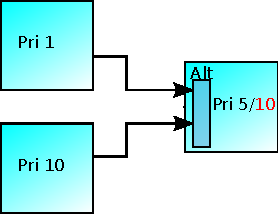
\includegraphics[scale=1.00]{images/alt-inheritance}
  \caption{Prioritetsnedarvning i \code{alternations.}}
  \label{fig:alt-inheritance}
  \end{center}
\end{figure}

\section{Implementering}\label{sec:deadline-implementation}
Vi vil i dette afsnit beskrive hvilke ændringer og tilføjelser vi skal foretage i \pycsp, for at implementere RTP. Ændringerne vil tage udgangspunkt i de emner, vi har diskuteret i foregående afnit med fokus på de problemstillinger der skal tages højde for ved implementeringen af dem.  
\subsection{Overskredne deadlines}
%Planlægning i realtime kræver at man tager stilling til, hvordan  overskredne deadlines skal håndteres. Enten kan det opfattes som en egenskab for processen hvor dens deadline enten kan være overholdt eller ej, eller også kan en overskreden deadline resultere i en exception.

%Hvilken metode, der egner sig bedst til RTP, afhænger af hvilken deadline, der er tilknyttet processen. Er der tilknyttet en soft deadline til en proces, vil processen stadig tilføje værdi til systemet, selvom det overskrider dens deadline. Derfor kan det stadig være bedst for systemet at fuldføre processen til ende. I dette tilfælde  skal systemet blot markere at dens deadline er overskredet, og senere må programmøren så manuelt håndtere den overskredne deadline. 

%Hvis en proces har tilknyttet  en hard deadline, vil en overskredet deadline ikke tilføje værdi til systemet, og derfor kan det ikke betale sig for systemet at lade processen blive færdig. Processen skal derfor stoppes hurtigst muligt, så systemet i stedet kan udføre de processer hvis deadline endnu ikke er overskredet. For et system, hvor processerne har hard deadlines, vil det derfor være bedst, hvis en overskredet deadline resulterer i en exception, der med det samme stopper processen, og lader programmøren bestemme hvordan processen skal forholde sig til at deadlinen er overskredet.

%Vi har valgt, at der i vores system skal kaldes en exception, hvis en deadline overskrides. Dette er gjort ud fra en betragtning om, at systemet ikke kender konsekvensen af en overskredet deadline, men på processniveau har udvikleren tilføjet en deadline, og derfor må det være udviklerens ansvar at håndtere processen ved en overskridelse af deadline.  Hvis processen stadig kan bidrage med værdi, kan programmøren lade processen fortsætte sin kørsel. Alternativt kan processen lukkes korrekt ned. Ulempen ved at kalde en exception er, at processen stopper sin eksekvering i utide, hvilket kan give problemer, f.eks. hvis processen er tilknyttet en kanal og venter på at kommunikere.  Kanalerne holder i \pycsp styr på antallet af processer, der vil kommunikere, og hvis processen pludseligt forsvinder vil tilstandsvariablerne ikke være sat korrekt. Det er derfor vigtigt at processen korrekt fjerne sig selv fra kanalen i forbindelse med en exception.
Vi har i foregående afsnit argumenteret for, at alle overskredne deadlines bør resultere i en exception. Dette er oplagt at implementere i \sched en, så det checkes ved kontekstskift, om en deadline for den proces der skiftes fra, er overskredet, og i givet fald, kaster en exception. Vi ønsker dog at få kastet vores exceptions så hurtigt som muligt, for derved at gøre opmærksom på den overskredne deadline. Derfor checker vi yderligere for overskredne deadlines, når der kommunikeres på en kanal, og når der foretages et valg i en \code{alternation}. 
\fxnote{Mere i dette afsnit ville være rigtig rart}

\subsection{Ændringer i \sched en}
\phantomsection
\label{sec:sched-changes}
I \code{greenlets}-versionen af \sched en findes der som nævnt i \cref{sec:scheduler} tre lister af processer: \code{new}, \code{next} og \code{timers}. De tre lister er prioriteret således, at der først kigges på processer fra \code{timers}, dernæst fra \code{new} og til sidst kigges der i \code{Next}.

I RTP er det ikke hensigtsmæssigt at inddele processerne i disse tre  kategorier. Vi skal derimod have et miljø, der gnidningsløst tillader processer både med og uden deadlines, samt at de dynamisk kan ændres. Skemaplanlæggeren skal i forbindelse med processkift hurtigt kunne finde den næste proces, der skal udføres.

Vi har derfor valgt at fjerne  de tre lister og erstatte dem  med \code{has"_priority},  \code{no"_priority} og \code{timers}. \code{has"_priority} og  \code{no"_priority}  benyttes til aktive processer, der ønsker at blive udført, mens \code{timers} er en kopi af \des versionen. 

Det er vigtigt at bemærke ifht. processer der ligger i \code{timers}, at udvikleren ikke kan forvente at de bliver aktiveret på de eksakte tidspunkt han har defineret. Dette er kun muligt i \des versionen hvor vi kan kontrollere tiden. Den eneste garanti der gives, når vi arbejder med realtid, er at de tidligst aktiveres på det angivne tidspunkt. I \code{greenlets}-versionen  aktiveres først processer fra \code{timers} listen. Dette gøres fordi processer i denne version kun kommer på denne liste via \code{timeout}-guarden. En udvikler vil forvente  at processen venter i præcist det tidsrum man har angivet for så at fortsætte. For at emulere dette krav om kun at vente et præcist tidsrum foretrækkes derfor processer fra denne liste fremfor processer der bare ønsker at bliver kørt. I RTP antages det, at der findes en mængde processer, der skal gennemføres inden en deadline, hvorfor de må kæmpe om CPU-tid. En proces, der har ventet i \code{timers} listen skal derfor ikke nødvendigvis udføres med det samme, da det hele tiden bør være den proces med den højeste prioritet der skal udføres, uafhængigt af processerne i \code{timers} hoben. Processerne, der ikke længere skal vente på timeout, bliver derfor planlagt og udvalgt på lige fod med andre processer der er klar til at blive udført. 

Til at implementere \code{has"_priority} bruger vi også en hob, men da modulet \code{heapq} kun understøtter min-hobe kan vi ikke lave en klassisk prioritetshob, da den skal kunne udtrække processen med maksimal prioritet. Vi har dermed to muligheder, enten kan vi lave vores egen implementering af en maks-hob, eller også kan vi ændre vores prioriteter internt, så en lav værdi angiver en høj prioritet. Med en egen implementering har vi en  logisk opbygning af prioriteter, men vi får ikke fordelen ved den underliggende implementering  direkte i C, som man opnår ved brug af modulet heapq. Vælger vi at bruge dette, skal vi invertere prioritetsbegrebet, så det er den laveste prioritet, der udvælges først. Dette viser  sig dog ikke at være et problem  i vores tilfælde, da vi ønsker at benytte os af en EDF algoritme og derfor nemt kan opnå den ønskede effekt ved at bruge en proces' deadline som dens prioritet. Her vil en lav deadline betyde, at processen snart skal være færdig, hvilket resulterer i en høj prioritet.
Vi kan derfor blot benytte en proces' deadline som dens prioritet og benytte en min-hob. 

%Hvis man i en fremtidig version ønsker at udvide vores \sched , så en udvikler kan tilknytte bruger-prioriteter til proceserne, kan det f.eks implementeres ved efterfølgende at ændre \sched ens prioritet. Dette vil resultere i at processen bliver opprioriteret ifh. til andre processer.

\subsection{Preempting}

Som vi har beskrevet i \cref{sec:rtp-pycsp}, kan  man risikere, at en proces med lav prioritet proces og kørselstid\fxwarning{``med lav prioritet og kørselstid'' hvad betyder det?} kan blokere for en proces med høj prioritet. 
Her konkluderede vi at det er udviklerens opgave at processen afgiver kontrol, og derfor skal det være nemt at afgive kontrollen for processen. Til dette har vi lavet funktionen \code{Release()}, der minder om \code{Yield} for \code{co-rutiner}.

Implementeringen er meget simpel og er blot en wrapperfunktion, da den underliggende funktionalitet allerede eksisterer. Den aktive proces stopper og bliver genplanlagt til senere kørsel af \sched en. Dermed lægges processen på den relevante kø, og  \sched en får mulighed for at vælge en ny proces der skal udføres. Er der ikke kommet nye processer, vil det stadig være den originale proces, der vælges og kan fortsætte sin kørsel. Hvis der derimod er ankommet en eller flere nye processer i mellemtiden, som har højere prioritet, vil disse blive valgt i stedet.

Problemet ved denne tvungne procesafgivelse er, at det kan tage lang tid at lægge processerne i en min\_hob, som vil være spildt, hvis den alligevel med det samme fjernes fra køen. Man vil derfor nok i en senere version kunne optimere hastigheden af \code{Release()}.

\subsection{Udvidelse af \code{Process}}
Hver proces skal kunne tilknyttes en deadline, som er et tidsstempel, der angiver det tidspunkt, som udvikleren ønsker at processen skal være færdig inden. 
Desuden skal hver proces tilknyttes en prioritet. Denne prioritet bruges af \sched en til at udvælge hvilken proces der skal eksekveres. I EDF er prioriteten og deadline for en proces som  den samme, og prioriteten er derfor også et tidsstempel.

I forbindelse med prioritetsnedarvning kan en proces midlertidigt få ændret sin prioritet, hvilket vi diskuterer yderligere i \cref{sec:deadline-implementation-priorityinheritance}. For at kunne adskille prioriteten, der ikke altid er sat af udvikleren, og en deadline, der altid er sat af udvikleren, har vi  valgt at holde de to variable adskilt. 

Når en proces bliver udvalgt til at arve en prioritet gennem prioritetsnedarvning, skal \sched en  planlægge processen ifht. den nye prioritet.
Den nye prioritet er også et tidsstempel, og hvis ikke processen er færdig, inden denne prioritet er overskredet, vil en anden proces' deadline være overskredet. 
Vi kan derfor vælge at \code{RTP} skal kaste en  \code{deadlineException},  hvis  prioriteten overskrides. Ved at kaste en \code{deadlineException} i processer hvor prioriteten er overskredet, kan udvikleren se præcist hvilken proces, der var aktiv, og dermed se hvorfor den originale proces også kaster en \code{deadlineException}. 

\CRef{fig:producer-worker-consumer} viser et tidsdiagram for et generator/arbejder/forbruger-netværk bestående af tre processer B$_1$, B$_2$ og B$_3$. B$_3$ har den højeste prioritet, og B$_2$ arver denne prioritet. Hvis B$_2$ også kaster en \code{deadlineException} vil det tydeligt fremgå for udvikleren, at det er B$_2$ der bærer skylden for, at B$_1$'s deadline ikke blev overholdt.

En anden begrundelse for at lade en nedarvet prioritet medføre en \code{deadlineException} er hvis processerne er afhængige af hinanden. I \cref{fig:producer-worker-consumer}  nedarver  arbejderprocessen(B$_2$) og generatorprocessen (B$_1$) en  prioritet fra forbrugerprocessen (B$_3$). Hvis denne deadline ikke nås, er det data som arbejderprocessen bearbejder ikke længere relevant, og arbejderprocessen kan med fordel stoppe det irrelevante arbejde. I eksemplet ville arbejderprocessen (B$_2$) kunne stoppe sit arbejde til tiden $t = 5$ i modsætning til at fuldføre arbejdet, og stoppe i tiden $t = 6$.

\begin{figure}
 \begin{center}
  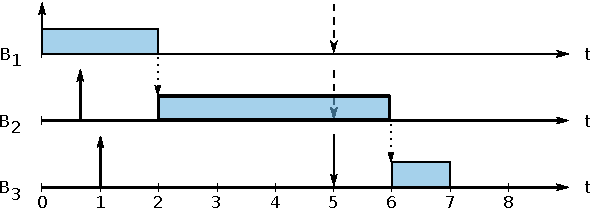
\includegraphics[scale=1.00]{images/producer-worker-consumer}
  \caption{Et generator/arbejder/forbruger -netværk. Kasserne repræsentere det tidsrum hvor processerne bliver bearbejdet. En pil op indikere hvornår processen er klar til at blive eksekveret. En pil ned indikere en deadline for processen. De stiplede pile i proces B$_1$ og B$_2$ til tiden t$=5$ viser en kunstig prioritet på baggrund af B$_3$'s deadline. Den lille stiplede pil mellem  B$_1$ og B$_2$ i t$=2$ og mellem B$_2$ og B$_3$ i t$=6$ viser kommunikation mellem processerne.}
  \label{fig:producer-worker-consumer}
  \end{center}
\end{figure}
\fxnote{Skriv på figurene hvem der er generator/arbejder/forbruger}
\begin{figure}
 \begin{center}
  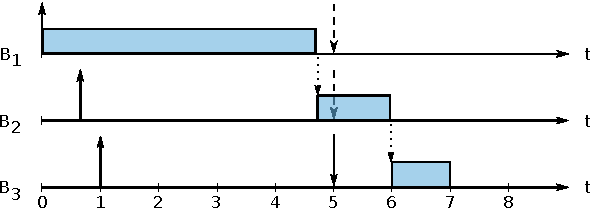
\includegraphics[scale=1.00]{images/producer-worker-consumer2}
  \caption{Samme netværk som i \autoref{fig:producer-worker-consumer}, men i dette tilfælde venter B$_2$  på data fra B$_1$ i hovedparten af tiden inden en deadline.}
  \label{fig:producer-worker-consumer2}
  \end{center}
\end{figure}


Der er dog ikke sikkert at en deadlineException i processer der har nedarvet en prioritet, er med til klarlægge hvilke processer der har brugt al tiden, og derfor bærer skylden for at en deadline ikke blev overholdt. \CRef{fig:producer-worker-consumer2} viser et eksempel på dette. Netværket er opsat som i \autoref{fig:producer-worker-consumer}, men i dette tilfælde bruger generatorprocessen (B$_1$) al tiden, og data bliver først sendt fra $B_1$ umiddelbart før en overskridelse af deadlinen. For en udvikler  vil det fremgå, som var det arbejderprocessen (B$_2$), der er ansvarlig for overskridelsen ligesom i \autoref{fig:producer-worker-consumer}, og ikke generatorprocessen $B_1$, som i dette eksempel brugte det meste af tiden. Dermed mister \code{deadlineException} sin troværdighed, og brugbarhed til at identificere hvor i netværket tiden bruges. 

Et andet problem ved at lade den aktive proces kaste en \code{deadlineException} er, at det vil pålægge udvikleren et væsentligt større arbejde med at håndtere disse exceptions. Såfremt vi implementerer det, kan enhver proces, der kan arve en prioritet via prioritetsnedarvning, kaste en exception. Det er ikke nødvendigvis klart gennemskueligt hvilke processer det vil være, hvorved udvikleren kan have svært ved at sikre ordentlig fejlhåndtering. Yderligere vil det medføre at excpetions kan kastes udenfor den kontekst de er relateret til, hvorved det kan være umuligt at håndtere dem korrekt.  

På baggrund af de opstillede fordele og ulemper, har vi valgt at kun processer med en eksplicit deadline, har mulighed for at kaste en \code{deadlineException}. Processer, der nedarver en prioritet, bliver planlagt i henhold til den højeste prioritet, de har, og vil altid  gøre arbejdet færdigt. En proces skal dermed kunne adskille sin egen deadline fra den prioritet, som den skal planlægges med, selv om de to værdier i en stor del af tiden vil være det samme.

En deadline er dermed en variabel der kun kan sættes af udvikleren og det er kun på baggrund af denne deadline at  processen skal kaste en \code{deadlineException}.

For at  \sched en kan udvælge processer introduceres prioritet, der som standard er det samme tal som deadlinen. For at kunne håndtere flere niveauer af prioritetsnedarvning,  gemmes prioriteten i en  liste kaldet \code{inherit\_priotity}. Denne liste af prioriteter  indeholder indledningsvis kun en prioritet som er deadlinen sat af udvikleren. Når andre processer  midlertidigt ønsker at ændre en proces' prioritet, tilføjes den til listen. Ved at bruge en liste i stedet for blot en variabel, har processen mulighed for at blive opprioriteret flere gange og derefter trinvist vende tilbage til de tidligere niveauer.

Når \sched en placerer processen i hhv. \code{has\_priority} og \code{no\_priority} hobene, bruges blot den mindste prioritet i listen af nedarvede prioriteter ihht. vores implementering af \sched en. Dette medfører, at når en proces efterfølgende  får ændret sin liste af prioriteter, skal processen genplanlægges for at sikre, at den placeres korrekt i min-hoben i \sched en. 

\subsection{Kanaler}
I \pycsp findes der kun kanaler af typen \code{Any-To-Any}, og derfor kan der altid  være et vilkårligt antal kanalender i hver ende af kanalen, der kan være klar til at kommunikere. Vi skal derfor foretage en ændring, så kommunikationen mellem kanalenderne altid foregår mellem de højst prioriterede processer. 

I greenletsversionen foregår udvælgelsen af kanalender til kommunikation ved hjælp af funktionen \code{match}, der udnytter at  hver kanal vedligeholder to lister af processer for hhv. de processer, der ønsker at sende, og modtage data på kanalen. Når en proces eks. ønsker at modtage data, tilføjer den sig selv til listen af processer, der ønsker at modtage, og prøver derefter i \code{match} funktionen at finde en proces, der vil sende data. Er der ingen processer, der venter på at sende data, venter processen på, at en proces melder sig klar til at sende data, ved at kalde \code{match}. Til hver vellykket kommunikation af data vil \code{match} altid blive kaldt to gange, hvor kun den sidste vil resultere i at kommunikationen lykkes.

Ideen bag funktionen \code{match} er enkel og  udnytter, at \code{greenlets}-versionen er enkelttrådet, så hver proces kan løbe listerne igennem, uden andre processer ændre på listernes tilstand.  Vi er kommet frem til, at  en simpel sortering af listerne ud fra processernes interne prioritet vil resultere i, at det altid er den højst prioriterede proces der indgår i kommunikationen. Den ændrede \code{match} kan ses i \cref{lst:match}, hvor det kun er linje 119 og 120 der er ændret.

\begin{lstlisting}[firstnumber=117 ,float=hbtp, label=lst:match, caption=Funktionen \code{match} der sorterer kanalrequests.]
def match(self):        
    if self.readqueue and self.writequeue:
        self.readqueue.sort(key=lambda channelReq:channelReq.process.internal_priority)
        self.writequeue.sort(key=lambda channelReq:channelReq.process.internal_priority)
        for w in self.writequeue:
            for r in self.readqueue:
                if w.offer(r):
                    return       
\end{lstlisting}

Funktionen \code{match} vil blive kaldt en gang for hver proces der ønsker at kommunikere, og derfor vil det kun være det sidste element i listen som ikke er sorteret korrekt ved hver kald af \code{match}. Desuden vil der altid i den ene liste maksimalt være på et element. Bemærk desuden at listerne er sorteret så værdien af den interne prioritet er stigende, og derfor er det processen med lavest værdi, der først bliver udvalgt til et match, i overensstemmelse med repræsentationen af prioriteter som nævnt i afsnittet ``Ændringer i \sched en'' %\vpageref{sec:sched-changes}.
på side \vpageref{sec:sched-changes}.
\fxerror{ret til vpageref}


\subsection{Prioritetsnedarvning}
\label{sec:deadline-implementation-priorityinheritance}
Prioritet i et RTP system skal ses i forhold til alle processers prioritet. En proces kan derfor ikke i sig selv have en absolut høj prioritet, men kun have høj prioritet ifht. de andre processers prioritet. Ved at give en høj prioritet til  en proces, vil dette dermed  indirekte sænke de andre processers prioritet, et fænomen vi vil kalde ``prioritetsdevaluering``.

For at minimere prioritetsdevaluering i forbindelse med prioritetsnedarvning, ønsker vi at minimere den tid en proces har en kunstigt høj prioritet, og at minimere antallet af processer, hvis prioritet øges. 

Som vi er kommet frem til i \cref{sec:rtp-pycsp-nedarvning}, skal  der foregå  prioritetsnedarvning i forbindelse med kommunikation, hvis der ikke findes nogle processer, der umiddelbart er klar til at kommunikere.  I \pycsp kan man umiddelbart evaluere, om der er processer klar til at kommunikere over en given kanal. Det skyldes, at processer der ønsker kommunikation befinder sig i listerne \code{readqueue} og \code{writequeue}. Hvis ingen processer ønsker at kommunikere, kan man dog ikke finde de processer som potentielt kan indgå i kommunikation.
Vi må derfor udvide kanalerne i RTP versionen med to lister, \code{readerprocesses} og \code{writerprocesses}, der består af de processer, der potentielt kan sende og modtage data over kanalen. Vi håndterer vedligeholdelsen af disse lister, ved at hver proces ved opstart tilføjer sig selv til de kanaler, den har mulighed for at kommunikere over. Et oplagt sted at implementere denne funktionalitet er i processens  \code{\_\_init\_\_}  funktion, da alle kanalender som denne proces potentielt kan kommunikere over, findes som argument til  \code{\_\_init\_\_} funktionen. \CRef{lst:process-init} viser udvidelsen af funktionen, hvor argumenterne gennemløbes, mens der ledes efter kanaler, som processen skal registreres i.

\begin{lstlisting}[firstnumber=29 ,float=hbtp, label=lst:process-init, caption=Uddrag af \code{Process}' \code{\_\_init\_\_}funktion]
for arg in args:
    if isinstance(arg, pycsp.greenlets.channelend.ChannelEndRead):
        arg.channel._addReaderProcess(self)
    if isinstance(arg, pycsp.greenlets.channelend.ChannelEndWrite):
        arg.channel._addWriterProcess(self)  
\end{lstlisting}

Kanaler kender nu  både de processer, der på et specifikt tidspunkt ønsker at kommunikere vha. listerne \code{readqueue} og \code{writequeue}, og de processer, der potentielt vil kunne kommunikere vha. listerne \code{readerprocesses} og \code{writerprocesses}. Processer der ønsker at kommunikere kan, som normalt umiddelbart evaluere om det er muligt; såfremt det ikke er muligt, kan den nu evaluere hvilke processers prioritet den kan øge, for at bringe dem i en tilstand hvor de kan indgå i den ønskede kommunikation. 

Funktionaliteten til prioritetsnedarvning skal implementeres i de to interne kommunikationfunktioner  \code{\_read} og \code{\_write}. Fordelen ved at placere prioritetsnedarvning i disse to funktioner er, at de bruges af processerne både i forbindelse med normal blokerende kommunikation og i forbindelse med kommunikation i \code{alternation}. Vi har udvidet funktionerne med følgende liste af begivenheder:
\begin{itemize}
\tightlist
	\item Undersøg om processen opfylder kriterierne for at starte en prioritetsnedarvning.
	\item Forhøj prioriteterne for de potentielle processer i enten \code{readerprocesses} eller \code{writer\-processes}.
	\item Umiddelbart efter kommunikationen nedprioriteres de processer, man midlertidigt har øget prioriteterne på.
\end{itemize}

Som beskrevet er det vigtigt, at vi igennem hele designet forsøger at begrænse mængden af prioritetsnedarvningen, og derfor har vi tilføjet en række egenskaber, der skal være indfriet, før prioritetsnedarvning forsøges. Disse er: processen skal have en prioritet, enten direkte eller efter en nedarvning; kanalen må ikke være klar til kommunikation, hvilket vil sige, at hvis processen ønsker at skrive, må der ikke findes en proces, der er klar til at modtage data; endeligt skal processen ikke have overskredet sin egen deadline, da denne til slut blot vil kaste en exception, og hele prioritetsnedarvningen vil være irrelevant.

Selve prioritetsforhøjelsen og den senere nedprioritering er simpel, da processen blot sender sin prioritet til alle processerne i den relevante liste dvs. \code{writerprocesses} for  \code{\_read} funktionen og vice versa. Hvis en proces modtager en lavere prioritet end dens egen prioritet, ses der bort fra hhv. op- og nedjusteringen, så en prioritetsnedarvning ikke resulterer i en forringelse af prioritet. 

\subsection{\code{Alternation}}

Som nævnt i afsnit \cref{misc:kanal-prioritet} har vi behov for at kunne tilknytte en prioritet til en kanal for at kunne håndtere udvælgelse i \code{alternations}. Vi har allerede prioriteter for processer og ønsker, at kanalernes prioritet skal defineres på baggrund af hvilke processer, der er tilknyttet kanalen. Vi skal kunne håndtere både input- og output-guards og ønsker seperate prioriteter for disse. Vi tilknytter derfor to prioriteter til hver kanal. De to prioriteter er sat som  de højst prioriterede processer, der er klar til at hhv. modtage og sende data. En kanals prioritet er derfor ikke fast som for processerne, hvor de får sat en prioritet (der dog kan ændres med prioritetsnedarvning), men nærmere en emuleret prioritet, som ændre sig baseret på alle processernes tilstand. 

Til at implementere de to prioriteter introduceres  to hjælpefunktioner, der løber hhv. \code{readqueue} og \code{writequeue} igennem og  finder den højst prioriterede proces, der er villig til hhv. at sende og modtage data. Når  \code{alternation} ønsker at finde prioriteten for en kanal, kigger den på om kanalen i \code{alternation} er tilknyttet en output- eller inputguard og finder den korrekte prioritet.


\section{Evaluering}
\subsection{Test af Korrekthed}
Vi har som i \des løbende skrevet test før vi implementerede hver ny funktion i \code{RTP}-versionen.  Tabellen herunder viser testresultaterne for de test der er lavet specifikt for \code{RTP}-versionen.
\begin{longtable}{lr}
   	\toprule
    \mc{Test} & \mc{Resultat} \\
    \midrule
    \endfirsthead 
    \toprule
    \mc{Test} & \mc{Resultat} \\
    \midrule
    \endhead % slut efterfølgende headere
    \bottomrule
    \multicolumn{2}{r}{\textit{fortsættes}}
    \endfoot % slut footer
    \bottomrule
    \endlastfoot % slut sidste footer
test\_Alternation  & ok\\
test\_AlternationChoiseReader  & ok \\
test\_AlternationChoiseWriter  & ok \\
test\_AlternationExecuteReadDeadline  & ok\\
test\_AlternationExecuteSkipDeadline  & ok\\
test\_AlternationExecuteTimeoutDeadline  & ok \\
test\_AlternationExecuteWriteDeadline  & ok \\
test\_Alternationchoise1Deadline  & ok \\
test\_Alternationchoise2Deadline  & ok \\
test\_ChoisemultipleReader  & ok \\
test\_ChoisemultipleReader2  & ok \\
test\_ChoisemultipleWriter  & ok\\
test\_PoisonAndDeadline1  & ok\\
test\_PoisonAndDeadline2  & ok\\
test\_Reader\_Inheritance  & ok\\
test\_RetireAndDeadline  & ok\\
test\_Writer\_Inheritance  & ok\\
test\_channelpriority\_from\_low\_deadline  & ok\\
test\_channelpriority\_from\_low\_deadline2  & ok\\
test\_channelpriority\_from\_no\_deadline  & ok\\
test\_channelpriority\_from\_no\_deadline2  & ok\\
test\_readDeadline  &ok\\
test\_writeDeadline  & ok\\
test\_xreset\_inheritance  & ok\\
test\_xreset\_inheritance\_from\_two\_step  & FAIL\\
\end{longtable}


 Alle test med en undtagelse fungerer korrekt. Testen der fejler hedder test"_xreset"_inheritance"_from"_two"_step, og viser en situation hvor den samme proces får løftets sin prioritet to gange i træk, først med en høj prioritet, og efterfølgende med en mellemprioritet. Efterfølgende skal processen sænke sin prioritet, først til  mellemprioriteten og tilslut til sin originale prioritet. Her viser det sig vi har lavet en fejl i implementeringen, således at prioriteten ikke bliver nedsat til mellemprioriteten. \CRef{fig:priority-inheritance} viser prioriteten mens processen bliver op og nedprioriteret. Tiden har ikke tilladt os at løse problemet, men  kan løses ved at kræve at, når en proces opprioriteres gemmes hvilken proces der står bag, så når en proces ønsker at fjerne sin opprioritering fra andre processer er det kun sin egen  prioritet den fjerner.  
 
  
\begin{figure}
 \begin{center}
  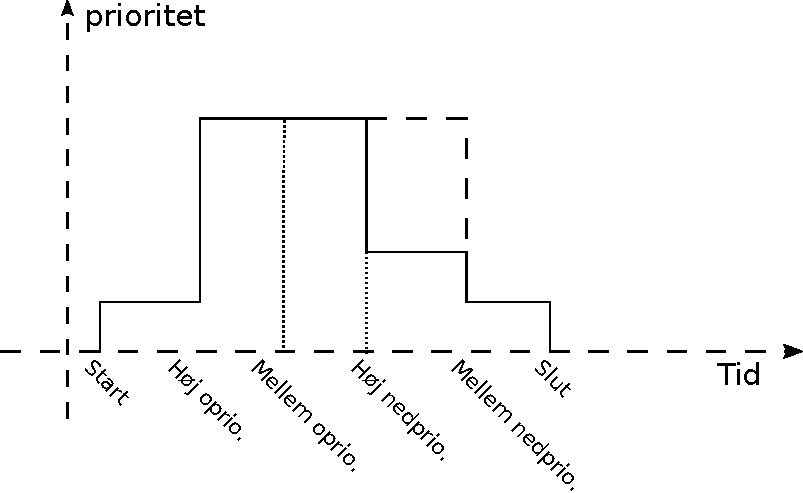
\includegraphics[scale=1]{images/priority-inheritance}
	\caption{Figuren viser hhv. forventet og faktisk prioritetsarvning. Der hvor den faktiske og forventede opførsel adskiller sig er forventet den fuldt optrukne streg, mens den stiplede streg er den faktiske opførsel.}
	\label{fig:priority-inheritance}
\end{center}
\end{figure}
  

\subsection{Slagterieksempel}

Først vil vi sammenligne de to udviklede versioner, for at se på deres fordele og ulemper, og til slut vi i dette afsnit sammenholde de to versioner, med et  eksempel der er implementeret i RTP-versionen.

Helt generelt opnår man når man ved brug af \pycsp et netværk, der nemt kan udvides hvis de fysiske rammer for slagteriet ændre sig. Viser det sig f.eks at kameraet holder den samlede produktivitet af netværket tilbage kan, slagteriet tilføjet endnu et kamera, og nemt udvide procesnetværket med endnu en kameraproces, som kan arbejde samtidigt med det første kamera. 

Forskellen i kode mellem \code{greenlets} og \code{proces}-versionen består af en linje, som indikerer hvilken version \pycsp skal bruge. En kørsel mellem de to versioner giver dog forskelligt resultat, som vist i \cref{tab:deadline-runs}. Dermed har valget af version betydning for både andelen af griseobjekter, der kan nå at blive bearbejdet, og hvor lang tid det tager i køre testen. Dette skyldes at testen køres på en multikerne CPU hvor \code{proces}-versionen dermed har mulighed for at køre parallelt. \code{Greenelts}-versionen derimod er begrænset til kørsel af en proces hvorfor der er flere grise der ikke når at blive bearbejdet inden for sin deadline.

\begin{table}[htbp]
	\centering
	\begin{tabular}{lrr}
       	\toprule
        \mc{Version} & \mc{Succesrate (\%)} & \mc{Tidsforbrug (s)} \\
        \midrule
        Greenlets & 42 & 16,5\\
        Processes & 71 & 10,3\\
        \bottomrule
    \end{tabular}
	\caption[]{Gennemførslen af simulation hvor 100 grise bliver sendt igennem procesnetværket. }\\
	\label{tab:deadline-runs}
\end{table}

Forskellen på kørselstiderne skyldes at detektoren venter på at aflevere griseobjektet til kameraet, og først når objektet er afleveret venter detektoren et normalfordelt tidsrum. Om dette er en urealistisk opførsel vil kræve mere domæneviden. Kan detektoren f.eks styre transportbåndet der fører grisene hen til detektoren er det en rimelig antagelse, mens det er urealistisk hvis båndet kører uafhængigt at detektoren.

I \code{procees}-versionen findes der fire processer og dermed kan der bearbejdes fire griseobjekter samtidigt. Dette sikre at det er de fire  griseobjekter nærmest robotten der arbejdes på, men samtidigt betyder det at man maksimalt kan arbejde på fire grise samtidigt. Ved at øge antallet af griseobjekter man kan arbejde på, vil man få mere tid per gris til at foretage de nødvendige beregninger. Man kan derfor vælge at tilføje flere konverterings og analyseprocesser, da disse ikke er bundet op på specialiseret hardware, og på den måde øge antallet af processer der kan arbejde samtidigt. Dette vil dog øge antallet af processer der må kæmper mod hinanden for CPU-tid, og griseobjekterne vil desuden skulle kæmpe mod hinanden for at komme igennem netværket uden hensyn til hvilken gris der er nærmest robotten. Man risikere dermed en starvation situation hvor griseobjekter svarende til  grise længere tilbage på transportbåndet overhaler griseobjekter længere fremme på transportbåndet.

\code{RTP}-udvidelsen bygger på \code{greenlets}-versionen, og vil derfor have de samme begrænsninger som denne, som diskuteret i implementeringen i afsnit \cref{sec:deadline-exampel-implementation}. Der er dog også en række fordele som vi vil komme ind på her.

Ved implementering af slagterieksemplet i \code{RTP}-versionen, slipper de enkelte processer for at holde styr på tiden, og vurdere om den enkelte gris deadline er overskredet. Når de modtager en gris sætter de deres egen deadline til grisens via funktionen \code{Set\_deadline}.  Hver proces skal i modsætningen til \code{greenlets}-versionen, kunne håndtere at modtage en \code{DeadlineException}, som de i dette eksempel blot kan håndteres ved at smide den nuværende griseobjekt væk. Det kan de gøre, da robotten på dette tidspunkt tager en beslutning uden specialviden om grisen, og griseobjektet er derfor ikke længere er relevant. I stedet kan processen  gå i gang med modtage et nyt griseobjekt.

I \code{greenlets}-versionen kom vi ind på at processerne frivilligt skal afgive kontrollen, før robotten kan foretage udskæringen, men at der ikke findes en metode til midlertidigt at afgive kontrollen. Med \code{RTP}-versionen og funktionen \code{Release} har alle processer mulighed for at afgive kontrollen så robotten rettidigt kan foretage selve udskæringen. Hermed skal vi ikke introducere en delt datastruktur.
  
selvom det var nødvendigt at basere RTP på  \code{greenlets}-versionen, medfører det at  kun en proces kan være aktiv på samme tid. Dermed kan vi kun udnytte en processor, som  passer dårligt sammen med denne applikation, som det ses af \cref{tab:deadline-runs}.  Vi kan dog til dels afhjælpe dette problem ved at udnytte at der i \code{greenlets}-versionen, findes en \code{IO}-dekorering. Denne dekorering placerer en funktion i en separat tråd, så flere funktioner kan køre samtidigt. Man skal her dog være opmærksom på at GIL'en stadig forhindre parallel udførsel. Eventuel parallel udførsel vil derfor kræve at koden i IO dekoreringen, kalder eksterne moduler som diskuteret i \cref{chap:csp}. Denne mulighed for parallel bearbejdning af flere processer vil dog  som i \code{processes}-versionen resultere i at processerne vil kæmpe mod hinanden om CPU-resurser. \code{RTP}-versionen har dog den store fordel at vi sikrer vi i modsætning til \code{proces}-versionen ikke risikere at griseobjekterne overhaler hinanden, men at netværket hele tiden har fokus på først at videresende griseobejektet nærmest robotten. \CRef{fig:pig-network3} viser hvordan netværket kan se ud med flere konverterings og analyse processer. 

\begin{figure}
 \begin{center}
  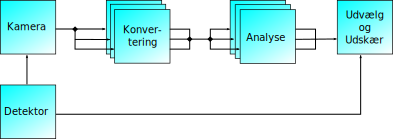
\includegraphics[scale=1]{images/pig-network3}
	\caption{Procesnetværk med flere konverteringsprocesser, og analyseprocesser}
	\label{fig:pig-network3}
\end{center}
\end{figure}

\section{Fremtidigt arbejde}\label{sec:deadlineFuture}
Vi har i dette kapitel opstillet en basal model for en RTP-implementering i \pycsp. Implementeringen er foretaget med henblik på blot at vise muligheden for en sådan model, og der er flere udviddelser som vi mener vil kunne forbedre modellen såfremt de kan implementeres. Vi vil i dette afsnit gennemgå nogle forbedringer som vi mener er interessante, men som ikke er inddraget i den basale implementering. 

\subsubsection{Evaluering af effektivitet}
Vi har med eksempler og test vist, at den implementerede løsning fungerer teoretisk korrekt. Vi har dog ingen reelle målinger af, hvor meget tid vi bruger på at evaluere hvilken proces der skal aktiveres, samt opretholde de metadata der skal til for at foretage denne vurdering. En grundig analyse af tidsforbruget i de administrative dele af vores implementering ville derfor være interessant at udføre, så man bl.a. kan udlede generelle retningslinier for, hvor ofte det vurderes hvilken proces der skal køre og hvor beregningstung hver proces bør være for at opnå den bedste ydelse. 

\subsubsection{Estimater for udførselstid}
Den primære begrænsning i vores løsning er manglen på at kunne evaluere hvor lang tid en proces eller dele af en proces tager at udføre. Hvis vi kunne udvikle en løsning der kunne foretage estimater af processers udførselstid ville vi kunne vælge en anden udvælgelsesalgoritme, som f.eks LL frem for EDF. Derved ville udvælgelsen af hvilken proces der skal aktiveres blive mere præcis. Ligeledes vil muligheden for at vurdere hvor langt en proces er nået i sin udførsel også være meget brugbart i forbindelse med prioritetsnedarvning. I vores implementering nedarver vi prioritet til alle processer som har mulighed for at opfylde en afhængighed. Såfremt vi kan vurdere hvilken proces der er tættest på at kunne opfylde afhængigheden, kan vi nøjes med at nedarve prioriteten til denne proces. Dette vil afhjælpe problemet med prioritetsdevaluering som nævnt i ``Ændring af prioritet'' i afsnit \ref{sec:aendring-af-prioritet}\vpageref{sec:aendring-af-prioritet}.

\subsubsection{Håndtering af forskellige typer deadlines}
I den nuværende løsning håndterer vi alle deadlines ens. Det er der fordele og ulemper ved, hvor en fordel er, at udvikleren får maksimal kontrol over hvad der skal ske såfremt en given deadline overskrides. Vi håndterer overskridelser af deadlines ved at kaste en exception når det sker. Dette er måske ikke altid ønskværdigt hvis det er en soft deadline der overskrides, da processen derved afbrydes. Det kunne tænkes at der er tilfælde hvor det er mere hensigtsmæssigt at udføre processen helt, og først her give besked om at den ikke nåede sin deadline.

%\fxerror*{Skal dette med}{I en fremtidig version ville man kunne udvide muligheden med en hybridversion, der skulle kunne håndtere processer med soft deadlines, der skal markeres, og kalde exceptions ved processer med hard deadline. Processen kunne f.eks have tilknyttet dens type af deadline. Systemet kan så reagere passende efter typen af deadlines, så soft deadlines blev færdigbehandlet, mens hard deadlines resulterede i en exception.}


\subsubsection{Udviklerbestemte prioriteter}
På nuværende tidspunkt har alle processerne den samme prioritet inden de planlægges, og deres prioritet afhænger udelukkende af deres deadline. Det kunne være interessant at undersøge om man kan bruge en anden skemaplanlægningsalgoritme, der kan håndtere at processerne har forskellige prioriteter inden de blev planlagt.

Hvis muligheden  for at differentiere processerne blev implementeret, kunne det være spændene hvis man kunne udvide \sched, så udvikleren kunne angive et kritisk sæt af processer, for hvilke det kunne garanteres at de ikke ville overskrider deres deadline. 

%\subsubsection{Implementering i andre \pycsp versioner}
%Det kunne være interessant at undersøge mulighederne for for at lave en implementering af RTP i andre versioner af \pycsp. Dette vil åbne op for de muligheder der er tilknyttet de forskellige implementeringer, hvilket vil gøre RTP mere praktisk anvendelig. Specielt er muligheden for brug af flere processorer med enten threads\footnote{Ved brug af eksterne moduler}- eller process-versionen. Dette vil dog, som tidligere nævnt, kræve at skemaplanlægningen flyttes til operativsystems skemaplanlægger og bliver derved 


%Test af effektivitet

%Estimater for kørselstid for processer

%Evaluering af hvor langt en proces er fra at være færdig

%Implemementering i process-version
\fxnote{Udvide kanaler til at være alternations med timeouts}

\section{Opsummering}

\chapter{Interaktiv planlægning}
\label{chap:is}
\fxwarning{Mangler Evaluering}
\fxwarning{Mangler Opsummering}
Interaktiv planlægning (\is) er det sidste anvendelsesområde vi vil belyse med henblik på at indføre tid i \pycsp. Det har dog vist sig at emnet kun er sparsomt berørt i litteraturen, og der er ikke en klar definition på hvad det er og hvor det anvendes. 
%og at de få definitioner af \is vi har fundet, ikke er et selvstændigt anvendelsområde, men en definition af RTP med en hard deadline uden at være et kritisk system. \cite{?}. 
Vi forventede at dette anvendelsesområde var brugt i forbindelse med computerspil, men efter at have studeret litteraturen, og have rådført os med Lektor Kenny Erleben, der underviser på Det Danske Akademi for Digital Interaktiv Underholdning (DADIU), er vi kommet frem til der ikke findes en udbredt definition af \is. Han fortæller desuden at en af begrundelserne for at computerspilfirmaerne ikke er interesseret i at oplyse om deres metoder til at planlægge begivenheder i spil, er at det  betragtes som en  virksomhedshemmelighed. 

Vi vil derfor i stedet på baggrund af en række praktiske eksempler indkredse hvad vi forventer \is skal kunne bruges til, og på baggrund af eksemplerne se på muligheden for at implementere en model, så eksemplerne kan implementeres i \pycsp. Dette kapitel adskiller sig dermed væsentligt fra de foregående to kapitler, i og med tidsmodellen ikke baserer sig på en fast definition givet af litteraturen og vi ikke bygger på kendt viden.

\section{Eksempler}
Vi har valgt to scenarier som vi forventer med fordel kan benytte \is. Det første er en repræsentation af et ur, hvilket vi mener er det simpleste eksempel der kan gøre brug af \is. Det andet eksempel er en del af et computerspil, som er vores forventede primære anvendelsesområde for \is. 

\subsection{Et ur}
Det første eksempel på \is er en repræsentation af et digitalur. Uret består af seks cifre, og en gang i sekundet skal sekunderne tælles op. Det er et  krav at en opdatering af uret skal sætte uret til at vise det korrekte tidspunkt. Vi forestiller os at uret er en del af et større system hvor der er andre ressourcekrævende begivenheder der er vigtigere at få udført end opdateringen af uret. Opdatering af uret foregår ved at planlægge en begivenhed til hvert sekund, der specificerer hvad uret skal vise. Da det har en lav prioritet, er der ikke er nogen garanti for at denne begivenhed indtræffer i det sekund den er planlagt til. Derfor skal begivenheden  bortkastes såfremt den overskrider sin deadline. Deadlinen vil være det når et nyt sekund begynder, for at sikre den krævede korrekthed. 

Uret er repræsentativt for \is da der planlægges en række begivenheder der skal foregå i fremtiden, og hvor hver begivenhed også har tilknyttet en deadline.

\subsection{Computerspil}
Et andet eksempel vi mener repræsenterer  \is, er mere realistisk og bunder i vores oprindelige forventning om at \is  var defineret af computerspilindustrien, som en metode til at planlægge hvordan spil kan forløbe. Uden deres definition af \is vil vi i stedet opstille et hypotetisk eksempel. 

Vi forstiller os et computerspil, der er skrevet i \pycsp og hvor hvert element i spillet er en selvstændig proces. I dette computerspil skal der være en fugl, der jævnligt flyver på tværs af skærmen. Fuglen skal starte på et givet tidspunkt og med en fast hastighed bevæge sig over skærmen. Fuglens flugt over skærmen udregnes af to typer processer, baseret på en model der minder om videokomprimering. Den første procestype, er en højprioritets proces der står for udregne positionen af fuglen med  et fast interval. Den anden procestype kan bestå af mange lavprioritetsprocesser. Hver lavprioritetsproces står for en egenskab ved fuglen, som  f.eks. at justere fuglen i forhold til dens position, optimere animationen af fuglen, tilknytte fuglekvidren og andre ikke essentielle egenskaber. Den højtprioriterede proces udføres sjældent men er essentiel at få udført, mens lavprioritetsprocesserne blot skal udføres hvis der er mulighed for det og ellers skal droppes.

Uden tab af generelitet vil vi i dette eksempel begrænse os til at fokusere på en høj og en lavprioritets proces. Højprioritetsprocessen står for at beregne positionen mens lavprioritetsprocessen står for at flytte fuglen i forhold denne position.

\section{Beskrivelse}
Ud fra eksemplerne kan vi se på hvilke egenskaber de har, og hvilke krav de derved stiller for at kunne håndteres i et programmeringssprog. Først og fremmest ligger det inden for realtid ligesom RTP. Ligeledes skal der være mulighed for at tilknytte en deadline til en begivenhed. Dette vil i vores opstillede eksempler være hard deadlines, men vi kan ikke udelukke at der findes eksempler hvor andre typer deadlines vil være fordelagtige. Eksemplet med computerspillet viser at der er behov for at tilknytte en prioritet, der er uafhængig af deadline, til en begivenhed. Dette har vi diskuteret som en mulig udvidelse til RTP i \cref{sec:deadlineFuture}. Disse egenskaber minder alle om dem der er er givet for RTP. Ud over disse skal vi også kunne tilknytte et starttidspunkt til en begivenhed. Det lægger sig mere op af \des med det forbehold at vi i \is ikke garanterer at en begivenhed sker på et bestemt tidspunkt, men tidligst på det angivne tidspunkt.  

Vi kan dermed se \is som en blanding af RTP og \des, med tidsmodellen og deadlines fra RTP, og startidspunkter fra \des. 

%\is arbejder ligesom RTP i realtid. Desuden minder de også om hinanden da man i begge modeller arbejder med begivenheder, der har tilknyttet deadlines. For det tredje viser computerspilseksemplet at en udvikleren skal kunne tilknyttes prioriteter til begivenheder, der skal sættes uafhængigt af deres deadline i \is. Dette nævnte vi som en mulig udvidelse til RTP i \cref{sec:deadlineFuture}.

%\is og \des minder også om hinanden da man i begge modeller skal kunne planlægge en begivenhed til at foregå ud i fremtiden. Men hvor \des kan garantere at begivenheden sker på præcist det angivne tidspunkt kan vi i \is kun garantere at det sker efter et givent tidspunkt.

\section{Design og implementering} 

Da kravene til \is rent praktisk ligger meget tæt op af de løsninger vi tidligere har beskrevet, i RTP, vil vi ikke implementere en selvstændig \code{\ip}-version der har et stort overlap med \code{RTP}-versionen. Vi vil i stedet udvide RTP-versionen med den krævede funktionalitet så RTP kan foretage både RTP og IP.
Vi skal derfor udvide RTP så man kan planlægge begivenheder der skal foregå ud i fremtiden, samt kunne sætte en prioritet på en proces uafhængigt at processens deadline. 

%I \des kom vi frem til at planlægningen af begivenheder ud i fremtiden også kan tolkes som en venten. Dermed kan man se på \is som en udvidelse til RTP, hvor man udover at have mulighed for at sætte en deadline skal have mulighed for at vente. For at kunne bruge RTP til \is vil det desuden være hensigtsmæssigt at  udvide RTP så det er muligt for udvikleren at tilknytte en prioritet til begivenheden.

\subsection{Funktionerne \code{Now} og \code{Wait}}

Vi argumenterer i kapitel \ref{chap:des} for at planlægning af begivenheder til et givet tidspunkt, kan tolkes som venten indtil tidspunktet. Vi vil derfor også i forbindelse med \ip, introducere de to globale funktioner \code{Now} og \code{Wait}, der hhv. returnerer den aktuelle tid og lader en proces vente i et givent tidsrum. Vi har ændret den interne implementering af funktionerne, så de bruger realtid. Ved at genbruge de samme funktioner, sikres en ensartet implementering af tid på tværs af TimedPyCSP, og man kan i vores øjne med fordel tilføje funktionen \code{Now} til alle \pycsp versionerne, for på den måde at ensrette de forskellige implementeringer. Hvis \code{Now} blev inkluderet i \code{greenlets}-versionen kunne den fjernes helt fra denne version, da de baserer sig på den samme tidsmodel nemlig realtid.

Forskellen i implementering mellem versionen der benytter realtid som tidsmodel ifh. til versionen der bruger diskrettid som tidsmodel er simpelt. I stedet at det er \sched en, der kender tiden, og derfor er dennes tid vi returnere i diskret tid, bruger vi nu Pythons \code{time}-modul. Genimplementeringen består derfor kun i at ændre funktionen \code{Now} til at bede \code{time}-modulet om det nuværende tidspunkt. 

\subsection{Udvikler"-prioriteter}
I computerspilseksemplet, har processerne forskellige prioritet dikteret af udvikleren. Denne prioritet er ikke det samme som den prioritet der allerede findes i RTP, da denne  er beregnet af \sched en. For at adskille dem vil vi kalde prioriteterne der er angivet af udvikleren for udvikler-prioritet. Vi skal udvide RTP således at det kan håndtere processer, der både kan have deadlines og udvikler"-prioriteter tilknyttet. Dette har vi allerede beskæftiget os med i \cref{sec:deadlineFuture}, som en fremtidsmulighed, og passer derfor godt sammen med RTP.

Først skal det fastlægges i hvilket interval udvikler-prioriteter kan antage. Vi ønsker ikke at begrænse udvikleren ved at have for få prioriteter, men omvendt reduceres \sched ens  mulighed for at udvælge processer hvis hver proces har sin egen unikke prioritet. Hvis en udvikler kan vælge mellem et stort antal prioriteter risikere man også at introducere en prioritetsskrue. Dette sker hvis en udvikler flere gange undervejs i udviklingen af et program øger den maksimale prioritet, da han mener sin nuværende proces er den vigtigste uden at gennemtænke det i relation til alle andre processer. Dermed risikere man at udvande prioriteten de allerede udviklede processer.  Der skal derfor være en maksimal prioritet, og intervallet man kan angive prioriteter i, må ikke være så stort at processerne for unikke prioriteter.

Præcis  hvor stort intervallet skal være for udvikler"-prioriteter, kræver dog en bredere analyse af flere projekter, og vi vil derfor begrænse os til at lave et foreløbigt interval på ti, man senere nemt vil kunne ændre baseret på en bedre analyse.


I \code{RTP}-versionen er \sched en en EDF algoritme, som kun planlægger processerne på basis af deres deadline. Vi kan derfor ikke bruge den samme skemaplanlægningsalgoritme, men skal udvide \sched en. For at udvide \sched en skal vi definere den indbyrdes relation mellem deadlines og udvikler"-prioriteter. Baseret på eksemplet kan vi se at de processer der har  tilknyttet en udvikler"-prioritet skal gå forud for både de processer der har tilknyttet en deadlines og dem uden noget. 

I RTP  indeholder \sched en alle processer med en prioritet i en enkelt hob kaldet \code{has\_priority}. Vi kan enten udvide denne hob til en liste af hobe, en for hver prioritet. Med en liste af hobe vil hver hob være mindre og dermed vil de enkelte operationer på hoben være hurtigere. \Sched en kan desuden bruge EDF på hver hob da alle processerne i hver hob har samme prioritet. Til at udvælge hvilken hob der skal udvælges en proces fra løbes listen igennem efter den hob med de højst prioriterede processer, der har elementer. 

Alternativt kan vi udvide den ene hob, der allerede findes så alle processer, både med og uden udvikler"-prioritet befinder sig i den samme hob. Med denne metode kan man ikke bruge EDF, men der skal udvikles en  funktion der kombinere  udvikler"-prioriteten og deadlinen, til en endelig prioritet. Man vil så kunne bruge en Least Priority First (LPF) algoritme, der fuldstændigt svare til EDF, men bruger prioritet til at basere udvælgelsen. I sagens natur vil denne hob  være større end hvis man brugte en liste af hobe. Dette er dog ikke et stort problem, da hoben gemme data i en træstruktur og  søgetiden vokser derfor logaritmisk til antallet af elementer. Vi antager derfor at forskellen mellem de to fremgangsmåder ikke vil være nævneværdig, og under alle omstændigheder, vil den ikke være anderledes end i \code{RTP}-versionen, hvor der også kun findes en hob. Fordelen ved kun at bruge en hob er at vi kan genbruge \code{has\_priority} hoben, og  ikke skal lave en større omskrivning af \code{RTP}-versionen. Desuden skal vi ikke lineært gennemløbe en liste af hobe for at finde den først hob med elementer, men kan med det samme starte i den korrekte hob. Endnu en fordel ved denne metode er at vi nemt kan  ændre vores oprindelige antagelse om at prioritet skal gå forud for deadlines, blot ved at ændre på den eksterne funktion der kombinere de to parametre.

Vi mener at fordelene ved kun at have en hob, og muligheden for at kunne ændre på vægtningen af forholdet mellem udvikler-prioritet er større end besparelsen i tid ved at have flere hobe der skal vedligeholdes. Derfor vælger vi  at genbruge bruge \code{has\_priority}, som den eneste hob til  processer der har deadlines og udvikler"-prioritet. Med kun en hob skal vi derfor udvikle en ekstern funktion der kombinerer to tal til en endelig prioritet. Det kombinerede tal skal have den egenskab altid at udvikler"-prioriteten har forrang. Hver at bemærke er at des højere udvikler-prioriteten er des vigtigere er processen. I implementeringen af \code{has\_priority} bruges der en min-hob, hvorfor vi internt invertere udvikler"-prioriteten, så 0 er den højeste prioritet, og processer, hvor udvikleren ikke har angivet en prioritet, sættes til 10.

Vi valgt at implementere en simpelt løsning, hvor  de to tal lægges efter hinanden. Hvis man eksempelvis har en udvikler"-prioritet på 2 og en deadline på 20, sættes de efter hinanden så den endelige prioritet bliver 220. Dette kan vi gøre da antallet af cifre i hhv. deadlines og udvikler-prioritet ligger fast, så vi ikke risikere en forskydning, når de ligges efter hinanden. For at sikre at processer der har en udvikler"-prioritet, men ingen deadline også kan planlægges, bruges der en kunstig høj deadline. Man vil i vores løsning nemt kunne ændre på måden hvordan de to tal kombineres, blot ved at ændre i en funktion. 


% dikterede valget af \sched at priorite


    
\section{Evaluering}
Vi har i det foregående afsnit beskrevet hvad der skal til, for at implementere \is i \pycsp. Vi vil i dette afsnit gennemgå hvordan \is kan implementeres, for derefter at evaluere vores løsning med udgangspunkt i ureksemplet.

Netværket er struktureret som vist i figur \cref{fig:watch_network}. Som vi kom ind på tidligere, har vi en ur-proces, en række tidsstempel-processer, og nogle dummy.processer. Ur-processen modtager et tidstempel fra alle  tidsstempel-procceserne, og står så for at  opdatere uret. Tidsstempel-processerne modtager fra start af hver sit tidsstempel og de står så for at vente indtil dette tidspunkt, for så at sende tidspunktet til ur-processen. Samtidigt med at uret tælles op køres der også en række dummyprocesser i par, som kommunikere med hinanden. Hver dummyproces udregner 50.000 iterationer i en simpelt estimering af \pi. På testmaskinen tager dette i gennemsnit 0.07707 sekunder med en SA på 0.01245 sekunder.

rDisse processer brugte vi også i RTP eksemplet, og skal vise at der foregå andet arbejde på maskinen. 
\begin{figure}
 \begin{center}
  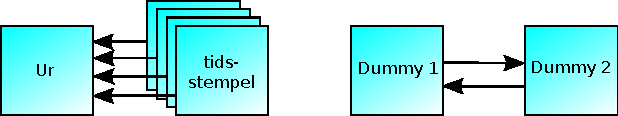
\includegraphics[scale=1]{images/watch-network}
	\caption{Procesnetværk med flere konverteringsprocesser, og analyseprocesser}
	\label{fig:watch_network}
\end{center}
\end{figure}

I \code{greenlets}-versionen skal tidsstempel-processerne vente på at kunne sende sit tidsstempel. Dette gør de ved at oprette en separat tråd  via \code{IO}-dekoratøren. I den separate tråd venter de via funktionen \code{sleep}. Dette er standardmetoden for \emph{greenlets}-versionen når processer ønsker at kunne vente uden at blokere for hele programmet, og er beskrevet på  hjemmesiden for \pycsp. Det medfører dog et overhead at skulle oprette en ny tråd blot for at vente.  Med introduktionen af \code{Wait}, bliver processen lagt på \code{timers}-hoben, og det er derfor ikke længere krævet at oprette en separat tråd til en proces der ønsker at vente. en udvikler der skal planlægge en proces til senere kørsel, slippe derfor i RTP for at skulle introducere \cref{fig:sleep} før en proces kan planlægges.

\begin{lstlisting}[firstnumber=1 ,float=hbtp, label=fig:sleep, caption=Funktion der venter et antal sekunder]
@io
def sleep(n):
    import time
    if n>0: time.sleep(n)
\end{lstlisting}
 
Ved implementeringen af \code{greelets}-versionen, opstår der et problem i opdateringen af uret. begrænsningen om kun at  opdatere uret så længe tidsstemplet er korrekt, har vi implementeret med en \code{alternation}, og en timeout.  Tidsstempel-processen, skal derfor inden et sekund have sendt beskeden til uret, og vil ellers helt droppe forsendelsen. Resultatet af denne implementering kan man se af linje 1 i \cref{tab:watch}. Den gennemsnitlige forsinkelse på 1.529 sekunder burde være umuligt, da opdateringer på over et sekund bør falde bort. Grunden til forsinkelsen ikke falder bort skyldes at tidsstempel-processen korrekt får overført tidsstemplet til urprocessen inden for et sekund. Ur-processen bliver efterfølgende lagt på \code{next} listen da den er klar til at blive kørt. Her skal den så slås med dummy-processerne for at blive udvalgt af \sched en. Når ur-processen bliver udvalgt er tiden forpasset og uret bliver opdateret for sent.
Vi har derfor lavet endnu en version hvor vi også ur-processen efter den har modtaget tidsstemplet kontrollere at tiden ikke er forpasset. Resultatet af denne ændring ses af linje 2 i tabellen, hvor vi kan se at ikke en eneste gang når uret at blive opdateret inden sekundet er forpasset.
\begin{table}[htbp]
	\centering
	\begin{tabular}{l>{\centering\arraybackslash}p{3.1cm}>{\centering\arraybackslash}p{3.1cm}>{\centering\arraybackslash}p{3.1cm}}
       	\toprule
        \mc{Version}     & Rettidige tidsopdateringer&Gennemsnitlig forsinkelse&Standard Afvigelse (SA)\\
        \midrule
        Greenlets ver. 1 & 0  & 1.529 & 0.276 \\
        Greenlets ver. 2 & 0  & NaN   & 0\\
        RTP              & 80 & 0.539 & 0.411 \\
        RTP (50 opdateringer) &100 & 0.077& 0.023\\
        \bottomrule
    \end{tabular}
	\caption[]{Proces-netværk betstående af et ur, 100 opdateringer, og baggrundsprocesser }\\
	\label{tab:watch}
\end{table}

De to forskellige implementeringer af \code{Greenlets}-versionen viser godt hvorfor den ikke er egnet til planlægge processer der er skal aktiveres inden for en tidsperiode. Problemet er at selvom tidsstempel-processerne sender sit data til ur-processen inden for tidsgrænsen. Skal denne stadig kæmpe om at blive aktiveret mod alle dummy-processerne. \Sched en aktiverer processerne ud fra en FIFO strategi, og ur-processen vil derfor komme sidst i køen der ønsker at blive aktiveret. 

I modsætning til \code{greenlets}-versionen, og dens FIFO strategi ser vi i tabellen for RTP-versionen at den  når 80\% af tidsstemplerne. I modsætning til Greenlets-versionen indeholder forsinkelsen kun de tidsstempler der ankom rettidigt. Det mest bemærkseslværdige ved RTP-versionen er SA. Den er meget høj og indikere dermed den gennemsnitlige forsinkelse variere meget. Dette passer ikke sammen med vores forventning om at watch-processen kommer til som den første proces. 


Ved at undersøge de forsinkelsen for de enkelte opdateringen, kunne vi se at de første opdateringerne ankom med en forventet forsinkelse, men igennem  kørte, steg forsinkelsen. Som alternativ til 100 opdatering prøvede vi derfor med 50 opdateringer, og fik et resultat som vi havde forventet. Forsinkelsen de ankommer med er svare til en kørslen af en dummyproces, hvilket er forventet da vi ikke har preemptiv kontekstskift, og derfor nødvendigvis må afslutte en dummyproces før tidsstempel-processen bliver aktiveret. Yderligere undersøgelse sted bestemmer vores problem til prioritetsnedarvning, nærmere bestemt at vi ikke korrekt får nedgraderet ur-processen igen. I dette tilfælde medvirker det til at de efterfølgende tidsstempel-processer fejlagtig modtager en prioritetsnedarvning. Det medfører at antallet af nedarvede prioriteter  hver tidsstempel proces modtager konstant øges.


\section{Konklusion}

%\begingroup
%\setsecnumdepth{part} 
\chapter{Konklusion} 
\label{chap:konklusion}

Vores mål med dette speciale, var at undersøge muligheden for at lave en udvidelse af \pycsp, der muliggør brugen af tid direkte i sproget. Der findes allerede et massivt teoretisk arbejde indenfor området, men ingen praktisk anvendelig implementeringer, så vores fokus har været på at det skulle være praktisk anvendeligt. Dette afspejles ved at vi har valgt at benytte eksempler som omdrejningspunkt for vores analyser af de tre anvendelsesområder. 

De tre anvendelsesområder vi identificerede i introduktionen var diskret simulering, realtids-planlægning og interaktiv tid. 

Indenfor diskret simulering har vi udviklet en løsning, der er let at anvende, og som eliminerer kravet om en delt datastruktur for at administrere tid i \pycsp. Løsningen kræver væsentligt mindre kode til at administrere tiden, end en tilsvarende løsning lavet i ren \pycsp.  




Tidsmodeller/anvendelsesområder


Praktisk anvendelig implementering


nuværende tilstand for anvendelsesområderne

DES



RTP



IP


%\endgroup 

 
%%%%%%%%%%%%%%%%%%%%%%%%%%%%%%%%%%%%%%%%%%%%%%%%%%%%%%%%%%%%%%%%%%%%%


\SingleSpacing
\fxwarning{Check at sidetallet på litteraturlisten passer}

\printbibliography[]
%\newpage
%\backmatter
%\appendix
%\chapter{Billag}

%\pagenumbering{roman}
%\restorepagenumber

%\chapter{Testresultater}
\thispagestyle{empty}

\section{Testresultater for \des}
\label{app:des-test}
\begin{longtable}{lr}
   	\toprule
    \mc{Test} & \mc{Resultat} \\
    \midrule
    \endfirsthead 
    \toprule
    \mc{Test} & \mc{Resultat} \\
    \midrule
    \endhead % slut efterfølgende headere
    \bottomrule
    \multicolumn{2}{r}{\textit{fortsættes}}
    \endfoot % slut footer
    \bottomrule
    \endlastfoot % slut sidste footer
    Doctest: simulation.Simulation & ok\\
    Doctest: simulation.io & ok\\
    Doctest: guard.testsuite & ok\\
    Doctest: alternation.Alternation & ok\\
    Doctest: alternation.testsuite & ok\\
    Doctest: channel.Channel & ok\\
    Doctest: channel.testsuite & ok\\
    Doctest: process.Parallel & ok\\
    Doctest: process.Spawn & ok\\
    Doctest: process.test\_suite & ok\\
    test\_alternation (test\_simulation.SimulationTestCase) & ok\\
    test\_buffer (test\_simulation.SimulationTestCase) & ok\\
    test\_buffered\_channels (test\_simulation.SimulationTestCase) & ok\\
    test\_decompose (test\_simulation.SimulationTestCase) & ok\\
    test\_io (test\_simulation.SimulationTestCase) & ok\\
    test\_timers1 (test\_simulation.SimulationTestCase) & ok\\
    test\_timers2 (test\_simulation.SimulationTestCase) & ok\\
    test\_timers3 (test\_simulation.SimulationTestCase) & ok\\
    test\_timers\_time\_in\_past (test\_simulation.SimulationTestCase) & ok\\
    test\_wait (test\_io.TestCase) & ok\\
\end{longtable}


\newpage
\section{Testresultater for RTP}
\label{app:rtp-test}
\fxnote{RS: ret stavefejl og sørg for at de to tabeller er formatteret ens}
\begin{longtable}{lr}
   	\toprule
    \mc{Test} & \mc{Resultat} \\
    \midrule
    \endfirsthead 
    \toprule
    \mc{Test} & \mc{Resultat} \\
    \midrule
    \endhead % slut efterfølgende headere
    \bottomrule
    \multicolumn{2}{r}{\textit{fortsættes}}
    \endfoot % slut footer
    \bottomrule
    \endlastfoot % slut sidste footer
test\_Alternation  & ok\\
test\_AlternationChoiseReader  & ok \\
test\_AlternationChoiseWriter  & ok \\
test\_AlternationExecuteReadDeadline  & ok\\
test\_AlternationExecuteSkipDeadline  & ok\\
test\_AlternationExecuteTimeoutDeadline  & ok \\
test\_AlternationExecuteWriteDeadline  & ok \\
test\_Alternationchoise1Deadline  & ok \\
test\_Alternationchoise2Deadline  & ok \\
test\_ChoisemultipleReader  & ok \\
test\_ChoisemultipleReader2  & ok \\
test\_ChoisemultipleWriter  & ok\\
test\_PoisonAndDeadline1  & ok\\
test\_PoisonAndDeadline2  & ok\\
test\_Reader\_Inheritance  & ok\\
test\_RetireAndDeadline  & ok\\
test\_Writer\_Inheritance  & ok\\
test\_channelpriority\_from\_low\_deadline  & ok\\
test\_channelpriority\_from\_low\_deadline2  & ok\\
test\_channelpriority\_from\_no\_deadline  & ok\\
test\_channelpriority\_from\_no\_deadline2  & ok\\
test\_readDeadline  &ok\\
test\_writeDeadline  & ok\\
test\_xreset\_inheritance  & ok\\
test\_xreset\_inheritance\_from\_two\_step  & FAIL\\
\end{longtable}



\chapter{Eksempler}
\section{Eksempler til \des}
\lstinputlisting[label=code_wator, caption=WaTor i simulerings-versionen]{../projects/wator/wator-des.py}
\lstinputlisting[label=code_simpel_bank, caption=Simpelt bankeksempel i simulerings-versionen]{../projects/bank/src/bank03.py}
\lstinputlisting[label=code_avanceret_bank, caption=Avanceret bankeksempel i simulerings-versionen]{../projects/bank/src/bank04.py}

\section{Eksempler til RTP}  
\lstinputlisting[label=code_slagteri, caption=Slagterieksemplet RTP-versionen]{../projects/porks-rtp/porks-rtp.py}
\section{Eksempler til IP}  
\lstinputlisting[label=code_ur, caption=Ureksemplet RTP-versionen]{../projects/watch-ip/watch.py}

 %Fjern %, så vedhæftes bilag (i final)
\end{document}
